\chapter{维数}

本章中，所有环均假定为交换环，所有代数均为结合的、交换的且含幺的。

设 A 为一个环。如果 a 是 A 的理想且 n 是负整数，我们规定 \(a^{n} = A\) 。对于 A 的每个素理想 p，记 \(\kappa(\mathfrak{p})\) 为局部环 \(A_{p}\) 的剩余域；它按典范方式同构于环 A/p 的分式域（II, § 3, no. 1, prop. 2）。如果 A 是局部的，记 \(m_{A}\) 为其极大理想，并记 \(\kappa_{A} = A/m_{A} = \kappa(m_{A})\) 为其剩余域。

设 \(\rho: A \to B\) 是一个环同态。记 \(^a\rho\) 为从 \(\operatorname{Spec}(B)\) 到 \(\operatorname{Spec}(A)\) 的连续映射，它由 \(\rho\) 诱导（II, § 4, no. 3）。按照（V, § 2, no. 1, def. 1），如果 q 是 p 在 \(^a\rho\) 下的像，即 \(\rho^{-1}(q) = p\)，则称 B 的素理想 q 位于 A 的素理想 p 之上。设 M 是一个 B-模；当把 M 看成 A-模时，始终指 A-模结构 \(\rho_*(M)\)，它由外部运算 \((a, m) \mapsto \rho(a).m\) 定义（A, II, p. 30）。

设 M 是一个 A-模。如果 U（分别为 V）是 A（分别为 M）的加法子群，则用 UV 或 U.V 表示由 uv（其中 \(u \in U\) 且 \(v \in V\)）生成的 M 的加法子群。如果 S 是 A 的子集，则用 SM 表示 M 的子模 \(\sum_{s \in S} sM\)；由 S 生成的 A 的理想等于 SA，且有 S.M = SM。

\section{环的克鲁尔维数}

\subsection{拓扑空间的克鲁尔维数}

定义 1. --- 设 I 是一个有序集。I 的一个非空有限全序子集称为 I 的一条链。设 c 是 I 的一条链；c 的最小元和最大元称为 c 的端点。整数 Card(c) - 1 称为 c 的长度。I 的子集集合上的包含关系在 I 的链集合上诱导出一个序关系。如果 I 中具有与 c 相同端点的链里 c 是极大的，则称链 c 是饱和的。

为了表示长度为 n 的链，我们常写作“链” \(i_{0} < \cdots < i_{n}\)，其中 \(i_{k}\) 是 c 的元素，并按从 0 到 n 的整数严格递增地编号。

设 X 是一个拓扑空间。我们在 X 的不可约闭子集集合（II, § 4, no. 1, def. 1）上赋予由包含关系定义的序关系。当我们说 X 的不可约闭子集的一条链时，始终指按此序关系的一条链。

定义 2. --- 我们称拓扑空间 X 的克鲁尔维数为 dim kr(X)，或简单记为 dim(X)，即 X 的不可约闭子集的链长集合在 \(\overline{\mathbf{R}}\) 中的上确界。

对于 X 中的每个点 x，我们称 \(\dim_{x}(X)\) 为 X 在 x 处的克鲁尔维数；它是 x 的开邻域的维数的下确界。

我们有 \(\dim(\emptyset) = -\infty\) 。另一方面，如果 X 非空，则 X 中任一点的闭包都是 X 的不可约闭子集（II, § 4, no. 1, prop. 2），因而 X 的维数或者是 +∞，或者是一个正整数。假设 X 是分离的且非空；那么 X 的每个不可约子集都退化为一点，且 X 的维数为 0。

\pandocbounded{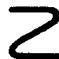
\includegraphics[keepaspectratio]{images/part001_0d60a61e.jpg}}

因此，对于分离空间，克鲁尔维数的定义没有什么意义，但它特别适合交换代数中遇到的拓扑空间（环的谱、*概形*、\ldots）。在本章中，不会与拓扑空间的其他维数概念（例如勒贝格维数）混淆，我们将简单地用“维数”表示“克鲁尔维数”。

命题 1. --- 设 X 是一个拓扑空间。

\begin{enumerate}
\def\labelenumi{\alph{enumi})}
\item
  如果 Y 是 X 的子空间，则有 \(\dim(\mathbf{Y}) \leqslant \dim(\mathbf{X})\)，且有 \(\dim_y(\mathbf{Y}) \leqslant \dim_y(\mathbf{X})\) 对 Y 的每个点 \(y\) 都成立。
\item
  设 \(x\) 是 \(X\) 的一个点，\(V\) 是 \(x\) 在 \(X\) 中的一个邻域。我们有 \(\dim_x(X) = \dim_x(V)\)。
\item
  设 \((\mathbf{X}_i)_{i\in I}\) 是 X 的闭子集的一个有限族，使得 \(\mathbf{X} = \bigcup_{i\in I}\mathbf{X}_i\)。我们有
\end{enumerate}

\(\dim(X) = \sup_{i \in I} \dim(X_i)\)且，对于每个点 \(x\)（属于 \(X\)），有 \(\dim_x(X) = \sup_{i \in J_x} \dim_x(X_i)\)，其中 \(J\) 表示满足 \(i \in J\) 且 \(x \in X\) 的指标集合。

其中  表示满足  的  的集合。\[
\mathrm{J} _ {x}
\]

证明 a)。如果 Z 是 Y 的不可约闭子集，则它在 X 中的闭包 \(\overline{Z}\) 是不可约的（II, § 4, no. 1, prop. 2），且有 \(\overline{Z} \cap Y = Z\)。因此，Y 的每条不可约闭子集链 \(c\) 通过在 X 中取闭包，定义了 X 的一条不可约闭子集链，其长度与 \(c\) 相同。由此得到不等式 \(\dim(Y) \leqslant \dim(X)\)。如果 U 是 X 中包含 Y 的一个点 \(y\) 的开子集，则有 \(\dim(U \cap Y) \leqslant \dim(U)\)，从而 \(\dim_y(Y) \leqslant \dim_y(X)\)。

证明 \(b\)。按定义 \(\dim_{x}(X) \leqslant \dim_{x}(V)\)，反向不等式由 \(a\)）得出。

证明 \(c\)。设 \(Z_{0} \subset \ldots \subset Z_{n}\) 是 X 的不可约闭子集的一条链。我们有 \(Z_{n} = \bigcup_{i \in I} (Z_{n} \cap X_{i})\)，且每个集合 \(Z_{n} \cap X_{i}\) 都在 \(Z_{n}\) 中闭；

由于 I 有限，\(Z_{n}\) 包含于某个 \(X_{i}\) 中。因此有 \(\dim(X) \leqslant \sup_{i} \dim(X_{i})\)，由 \(a\)）即得等式。

现在设 \(x\) 是 \(X\) 的一个点，且 \(n = \sup_{i \in J_x} \dim_x(X_i)\)，其中 \(J_x\) 如命题中所述。由 \(\dim_x(X) \geqslant n\) \(a\)）；为证明等式，不妨设 \(n\) 有限。对每个 \(i \in J_x\)，取 \(U_i\) 为 \(x\) 在 \(X\) 中的一个开邻域，使得 \(\dim(U_i \cap X_i) \leqslant n\)。置 \(U = (\bigcap_{i \in J_x} U_i) \cap (\bigcap_{i \in I - J_x} \complement X_i)\)；集合 \(U\) 在 \(X\) 中是开集。此外，由上一段有 \(\dim(U) = \sup_{i \in J_x} \dim(U \cap X_i) \leqslant n\)，从而 \(\dim_x(X) \leqslant n\)。

推论。--- a) 拓扑空间 X 的维数是其不可约分支的维数的上确界（II, § 4, no. 1, definition 2）。

\begin{enumerate}
\def\labelenumi{\alph{enumi})}
\setcounter{enumi}{1}
\tightlist
\item
  设 \(x\) 是 \(X\) 的一个点。我们有 \(\dim_x(X) \geqslant \sup_i \dim_x(X_i)\)，其中 \(X_i\) 遍历族。
\end{enumerate}
包含 x 的 X 的不可约分支族；如果 x 有一个仅含有限个不可约分支的邻域 V，则有等式（例如 V 为诺特空间时就是如此）。


第一条断言是直接的，因为 X 的不可约闭子集链正是 X 的不可约分支的不可约闭子集链（II, § 4, no. 1, prop. 5）。不等式 \(\dim_x(X) \geqslant \sup_i \dim_x(X_i)\) 由

命题 1 a) 得出。设 V 是 x 的一个仅含有限个不可约分支的邻域，令 \((\mathrm{V}_{j})_{j\in\mathbb{J}}\) 为包含 x 的 V 的不可约分支族。由命题 1 b) 和 c) 可得

\[
\dim_ {x} (X) = \dim_ {x} (V) = \sup _ {j \in J} \dim_ {x} (V _ {j});
\]

我们只需注意，每个 \(V_{j}\) 都包含于某个 \(X_{i}, i \in J_{x}\)，因而有 \(\sup_{j \in J} \dim_{x}(V_{j}) \leqslant \sup_{i \in J_{x}} \dim_{x}(X_{i})\)，于是得到结论。

命题 2. — 设 X 是一个拓扑空间。我们有 \(\dim(X) = \sup_{x \in X} \dim_x(X)\)。

事实上，按定义，有 \(\dim(X) \geqslant \dim_x(X)\) 对每个 \(x \in X\) 都成立。另一方面，如果 \(Z_0 \subset \ldots \subset Z_n\) 是 \(X\) 的不可约闭子集链，则对所有 \(x \in Z_0\) 以及 \(U\)（\(x\) 的每个开邻域），集合 \(Z_0 \cap U, \ldots, Z_n \cap U\) 构成 \(U\) 的不可约闭子集链（II, § 4, no. 1, prop. 7）。因此有 \(\dim_x(X) \geqslant n\)，从而 \(\dim(X) \leqslant \sup_{x \in X} \dim_x(X)\)。

推论。— 如果 \((\mathrm{X}_{\alpha})_{\alpha\in\mathbf{A}}\) 是拓扑空间 X 的一个开覆盖或局部有限闭覆盖，则有

\[
\dim (X) = \sup _ {\alpha \in A} \dim (X _ {\alpha}).
\]

只需证明，对于每个点 \(x\)（属于 \(X\)），有 \(\dim_x(X) = \sup_{\alpha \in A_x} \dim_x(X_\alpha)\)，其中 \(A_x\) 是由满足 \(\alpha \in A\) 且 \(x \in X_\alpha\) 的指标组成的集合。开覆盖的情形显然；局部有限闭覆盖的情形则由命题 1 c) 得出。

\subsection{闭子集的余维数}

定义 3. --- 设 X 是一个拓扑空间。

\begin{enumerate}
\def\labelenumi{\alph{enumi})}
\item
  如果 Y 是 X 的闭不可约子集，则称 Y 在 X 中的余维数为所有以 Y 为最小元的 X 的不可约闭子集链的长度在 \(\overline{\mathbf{R}}\) 中的上确界。
\item
  如果 Y 是 X 的闭子集，则称 Y 在 X 中的余维数，并记为 \(\text{codim}(Y, X)\)，为 Y 的不可约分支在 X 中的余维数在 \(\overline{\mathbf{R}}\) 中的下确界。
\end{enumerate}

注。--- 1) 因此，X 的闭子集 Y 的余维数是 Y 的不可约闭子集的余维数的下确界。我们有 \(\mathrm{codim}(\emptyset, \mathrm{X}) = +\infty\)；如果 X 非空，则 \(\mathrm{codim}(\mathrm{X}, \mathrm{X}) = 0\)。X 的每个非空闭子集都含有一个不可约闭子集（II, § 4, no. 1, prop. 5）；因此，闭子集 Y 在 X 中的余维数总是一个非负整数或 \(+\infty\)。当且仅当 Y 含有 X 的一个不可约分支时，它为零。

\begin{enumerate}
\def\labelenumi{\arabic{enumi})}
\setcounter{enumi}{1}
\tightlist
\item
  如果 Y 是 X 的非空闭子集，则 codim(Y, X) ≤ dim(X)。此外，dim(X) = sup codim(Y, X)，其中 Y 遍历不可约闭子集的集合。
\end{enumerate}

如果 Y 和 Y' 是 X 的两个闭子集且 Y' ⊂ Y，则 codim(Y, X) ≤ codim(Y', X)。

\begin{enumerate}
\def\labelenumi{\arabic{enumi})}
\setcounter{enumi}{2}
\tightlist
\item
  设 Y 是拓扑空间 X 的一个闭子集，且 \((\mathrm{X}_{\alpha})_{\alpha\in\mathrm{A}}\)（分别为 \((\mathrm{Y}_{\beta})_{\beta\in\mathrm{B}}\)）是 X（分别为 Y）的不可约分支族。对每个 \(\beta\in B\)，记 \(\mathrm{A}(\beta)\) 为由满足 \(\alpha\in A\) 且 \(Y_{\beta}\subset X_{\alpha}\) 的指标组成的集合。由于 X 的每个不可约子集都包含于某个 \(X_{\alpha}\) 中（II, § 4, no. 1, prop. 5），由定义 3 得：
\end{enumerate}

\[
\operatorname{codim} (Y, X) = \inf _ {\beta \in B} \sup _ {\alpha \in A (\beta)} \operatorname{codim} (Y _ {\beta}, X _ {\alpha}).
\]

\begin{enumerate}
\def\labelenumi{\arabic{enumi})}
\setcounter{enumi}{3}
\tightlist
\item
  设 \((\mathbf{Y}_i)_{i\in I}\) 是 X 的闭子集的一个有限族，且 \(\mathbf{Y} = \bigcup_{i\in I}\mathbf{Y}_i\)；有
\end{enumerate}

\[
\operatorname{codim} (\mathrm{Y}, \mathrm{X}) = \inf _ {i \in \mathrm{I}} \operatorname{codim} (\mathrm{Y} _ {i}, \mathrm{X}).
\]

事实上，Y 的每个不可约分支都包含于某个 \(Y_{i}\) 中。

命题 3. --- 设 X 是一个拓扑空间。

\begin{enumerate}
\def\labelenumi{\alph{enumi})}
\tightlist
\item
  对 X 的每个非空闭子集 Y，都有
\end{enumerate}

\[
\dim (\mathrm{Y}) + \operatorname{codim} (\mathrm{Y}, \mathrm{X}) \leqslant \dim (\mathrm{X}).
\]

\begin{enumerate}
\def\labelenumi{\alph{enumi})}
\setcounter{enumi}{1}
\tightlist
\item
  如果 Y、Z、T 是 X 的闭子集且 Y ⊂ Z ⊂ T，则
\end{enumerate}

\[
\operatorname{codim} (\mathrm{Y}, \mathrm{Z}) + \operatorname{codim} (\mathrm{Z}, \mathrm{T}) \leqslant \operatorname{codim} (\mathrm{Y}, \mathrm{T}).
\]

只需证明断言 \(a)\)，在 \(\dim(X)\) 有限的情形下。此时，\(\dim(Y)\) 和 \(\operatorname{codim}(Y, X)\) 均有限。存在一条 \(Y_0 \subset \ldots \subset Y_n\) 的 \(Y\) 的不可约闭子集链，长度为 \(n = \dim(Y)\)，以及一条 \(Y_n \subset \ldots \subset Y_{n+p}\) 的 \(X\) 的不可约闭子集链，长度为 \(p \geqslant \operatorname{codim}(Y, X)\)。由此 \(\dim(X) \geqslant n + p\)，从而得到结论。为证明 \(a)\)\(b)\)，可假设 \(Y\) 不可约。由于有 \(\operatorname{codim}(Y, Z) \leqslant \operatorname{codim}(Y, T)\)，当 \(\operatorname{codim}(Y, Z) = +\infty\) 时不等式成立。否则，设 \(Z_0\) 是 \(Z\) 的一个不可约分支，包含 \(Y\)，且满足 \(\operatorname{codim}(Y, Z) = \operatorname{codim}(Y, Z_0)\)。有 \(\operatorname{codim}(Z, T) \leqslant \operatorname{codim}(Z_0, T)\)，并且如上可见，\(\operatorname{codim}(Y, Z_0) + \operatorname{codim}(Z_0, T) \leqslant \operatorname{codim}(Y, T)\)，从而 \(b)\)。

定义 4. --- 如果对 X 的每一对满足 Y ⊂ Z 的不可约闭子集 (Y, Z)，以 Y 和 Z 为端点的每条不可约闭子集饱和链的长度都等于 codim(Y, Z)，则称拓扑空间 X 为串联的。

等价地说，对于 X 的每一对满足 codim(Y, Z) 有限的不可约闭子集 (Y, Z)，以 Y 和 Z 为端点的所有饱和链具有相同长度；而对于满足 codim(Y, Z) = +∞ 的每一对 (Y, Z)，不存在以 Y 和 Z 为端点的饱和链。

串联空间的每个闭子空间都是串联的。一个空间为串联的，当且仅当它的不可约分支都是串联的。

命题 4. --- 设 X 是一个拓扑空间。X 为串联的，当且仅当对 X 的每个满足 Y ⊂ Z ⊂ T 的不可约闭子集三元组 (Y, Z, T)，都有：

\[
\operatorname{codim} (\mathrm{Y}, \mathrm{T}) = \operatorname{codim} (\mathrm{Y}, \mathrm{Z}) + \operatorname{codim} (\mathrm{Z}, \mathrm{T}).
\]

设 X 是串联的。根据命题 3 b)，只需在 codim(Y, Z) 和 codim(Z, T) 均有限时证明该关系。将一条以 Y 和 Z 为端点、长度为 codim(Y, Z) 的不可约闭子集饱和链，与一条以 Z 和 T 为端点、长度为 codim(Z, T) 的不可约闭子集饱和链首尾相接，便得到一条以 Y 和 T 为端点、长度为 codim(Y, Z) + codim(Z, T) 的饱和链。但是，由于 X 是串联的，这个长度必然等于 codim(Y, T)。

反之，假设有 \(\operatorname{codim}(\mathbf{Y},\mathbf{T})=\operatorname{codim}(\mathbf{Y},\mathbf{Z})+\operatorname{codim}(\mathbf{Z},\mathbf{T})\)，并且该等式对满足 \(\mathbf{Y}\subset\mathbf{Z}\subset\mathbf{T}\) 的所有不可约闭子集均成立；我们证明 X 是串联的。为此，我们对整数 \(n\geqslant0\) 作归纳，证明对于 X 的每条不可约闭子集饱和链 \(Z_{0}\subset\ldots\subset Z_{n}\)，都有 \(\operatorname{codim}(Z_{0},Z_{n})=n\)。当 \(n=0\) 时显然成立。设 \(n>0\)，并假设长度 \(\leqslant n-1\) 的链都满足该性质。如果 \(Z_{0}\subset\ldots\subset Z_{n}\) 是长度为 \(n\) 的饱和链，则 \(Z_{0}\subset\ldots\subset Z_{n-1}\) 是长度为 \(n-1\) 的饱和链，因而 \(\operatorname{codim}(Z_{0},Z_{n-1})=n-1\)。根据关于 X 的假设，有 \(\operatorname{codim}(Z_{0},Z_{n})=\operatorname{codim}(Z_{0},Z_{n-1})+\operatorname{codim}(Z_{n-1},Z_{n})=(n-1)+1=n\)。

推论。— 设 X 是一个有限维不可约拓扑空间。X 为串联的，当且仅当对 X 的每一对满足 Y ⊂ Z 的不可约闭子集 (Y, Z)，有 codim(Y, X) = codim(Y, Z) + codim(Z, X)。

由命题 4，必要性成立。反之，假设该条件成立，并记 \(c(Z)\) 为整数 \(\operatorname{codim}(Z,X)\)，其中 \(Z\) 遍历 \(X\) 的每个不可约闭子集。如果 \(Y,Z,T\) 是 \(X\) 的三个不可约闭子集，且 \(Y\subset Z\subset T\)，则有

\[
\begin{array}{r l} \operatorname{codim} (\mathrm{Y}, \mathrm{Z}) + \operatorname{codim} (\mathrm{Z}, \mathrm{T}) & = (c (\mathrm{Y}) - c (\mathrm{Z})) + (c (\mathrm{Z}) - c (\mathrm{T})) \\ & = c (\mathrm{Y}) - c (\mathrm{T}) \\ & = \operatorname{codim} (\mathrm{Y}, \mathrm{T}), \end{array}
\]

且由命题 4，X 是串联的。

命题 5. — 设 X 是一个有限维拓扑空间。假设 X 的所有不可约闭子集极大链具有相同长度。则 X 是串联的；对 X 的每个不可约闭子集 Z，有

\[
\operatorname{codim} (Z, X) = \dim (X) - \dim (Z);
\]

对 X 的每一对满足 Y ⊂ Z 的不可约闭子集 (Y, Z)，有

\[
\operatorname{codim} (\mathrm{Y}, \mathrm{Z}) = \dim (\mathrm{Z}) - \dim (\mathrm{Y}).
\]

设 Y 和 Z 是 X 的两个不可约闭子集且 \(Y \subset Z\)。设 \(Y_{0} \subset \ldots \subset Y_{p}\) 是一条满足 \(Y_{p} = Y\) 且 \(p = \dim(Y)\) 的链，\(Z_{0} \subset \ldots \subset Z_{q}\) 是一条满足 \(Z_{0} = Z\) 且 \(q = \text{codim}(Z, X)\) 的链。对于每条满足 \(T_{0} \subset \ldots \subset T_{r}\)、\(T_{0} = Y\) 且 \(T_{r} = Z\) 的饱和链，该链

\[
\mathrm{Y} _ {0} \subset \dots \subset \mathrm{Y} _ {p - 1} \subset \mathrm{T} _ {0} \subset \dots \subset \mathrm{T} _ {r} \subset \mathrm{Z} _ {1} \dots \subset \mathrm{Z} _ {q}
\]

它是极大的，且长度为 \(p + q + r\)；根据关于 X 的假设，有 \(p + q + r = \dim(X)\)。令 \(r = \dim(X) - \dim(Y) - \text{codim}(Z, X)\)。由此 X 是串联的，并且对于上述 Y、Z，有

\[
\dim (\mathrm{Y}) + \operatorname{codim} (\mathrm{Y}, \mathrm{Z}) = \dim (\mathrm{X}) - \operatorname{codim} (\mathrm{Z}, \mathrm{X}).
\]

取 Y = Z，可见第二项等于 dim(Z)，从而得到命题。

\subsection{环的维数与理想的高度}

定义 5. —（交换）环 A 的克鲁尔维数，或简称维数，是拓扑空间  的克鲁尔维数，记为  （II, § 4, no. 3, definition 4）。如果  是 A 的素理想，则 A 在 \_ 处的维数记为 ，即 \_。

映射 \(\mathfrak{p} \mapsto \mathrm{V}(\mathfrak{p})\) 是从 A 的素理想集合到 \(\operatorname{Spec}(A)\) 的不可约闭子集集合的一个反序双射（同上，命题 14 的推论 2）。因此，A 的维数是 A 的素理想链的长度集合的上确界；它等于 \(-\infty\)、\(+\infty\) 或一个正整数。

设 \(\mathfrak{p} \in \operatorname{Spec}(\mathbf{A})\)；集合 \(\operatorname{Spec}(\mathbf{A})_f\)（其中 \(f\) 遍历 A）构成 \(\operatorname{Spec}(\mathbf{A})\) 的拓扑基，并且 \(\mathfrak{p}\) 属于开集 \(\operatorname{Spec}(\mathbf{A})_f\) 当且仅当 \(f\) 不属于 \(\mathfrak{p}\)。因此，\(\dim_{\mathfrak{p}}(\mathbf{A})\) 是数 \(\dim(\mathbf{A}_f)\) 的下确界，其中 \(f\) 遍历 \(\mathfrak{p}\)（II, § 5, no. 1, 命题 1）。

例。--- 1) 当且仅当 A 退化为 0 时，我们有  。要使 \textless 成立，必要且充分条件是 A 的每个素理想都是极大理想。维数为 0 的整环就是域。当且仅当它是阿廷环时，诺特环的维数为 {}（IV, § 2, no. 5, prop. 9）。

\begin{enumerate}
\def\labelenumi{\arabic{enumi})}
\setcounter{enumi}{1}
\item
Dedekind 环是维数 \(\leqslant 1\) 的诺特整闭环（VII, § 2, no. 2, th. 1）。更一般地，根据 V, § 1, no. 2, 命题 9 的推论 2，一个环是 Dedekind 环的有限直积，当且仅当它是诺特的、约化的、在其全分式环中整闭的且维数 \(\leqslant 1\)。
\item
如果 A 是一个赋值环（VI, § 1, No. 2, 定义 2），则其维数等于该赋值的高度（VI, § 4, No. 4, 命题 5）。
\item
设 A 是一个环。我们有
\end{enumerate}

\[
\dim (\mathrm{A} [ \mathrm{X} ]) \geqslant \dim (\mathrm{A}) + 1.
\]

事实上，如果 \(\mathfrak{p}_0 \subset \ldots \subset \mathfrak{p}_n\) 是 A 的素理想链，长度为 \(n\)，则我们得到 A[X] 的素理想链 \(\mathfrak{p}_0' \subset \ldots \subset \mathfrak{p}_{n+1}'\){}{}，其长度为 \(n+1\)，其中规定 \(\mathfrak{p}_i' = \mathfrak{p}_iA[X]\)（\(0 \leqslant i \leqslant n\)），以及 \(\mathfrak{p}_{n+1}' = \mathfrak{p}_nA[X] + XA[X]\)。

同样的论证给出不等式 \(\dim(\mathrm{A}[[\mathrm{X}]]) \geqslant \dim(\mathrm{A}) + 1\)。由此归纳得到不等式

\[
\begin{array}{l} \dim (\mathrm{A} [ \mathrm{X} _ {1},..., \mathrm{X} _ {n} ]) \geqslant \dim (\mathrm{A}) + n, \\ \dim (\mathrm{A} [ [ \mathrm{X} _ {1},..., \mathrm{X} _ {n} ] ]) \geqslant \dim (\mathrm{A}) + n. \end{array}
\]

稍后（§ 3, no. 4, 命题 7 的推论 3 以及命题 8 的推论 3）我们将证明，当 A 为诺特环时，前面两个公式中的等号成立。

* 5) 设 X 是一个复解析流形。如果 X 在 X 的一点 x 处具有复维数 n，则 X 上 x 处解析函数芽的局部环的维数为 n。*

\begin{enumerate}
\def\labelenumi{\arabic{enumi})}
\setcounter{enumi}{5}
\item
设 \(k\) 是一个域，A 是一个非零整 \(k\)-代数。则有 \(\dim(A) = 0\)。这由 V, § 2, no. 1 的命题 1 的推论以及 \(\dim(k) = 0\) 这一事实得出。
\item
如果 n 是 A 的幂零理想，则 Spec(A) 与 Spec(A/n) 同胚（II, § 4, no. 3, 注记）。因此有 dim(A/n) = dim(A)；特别地，如果 A\(_{red}\) 是环 A 除以其幂零根得到的商环，则有 dim(A) = dim(A\(_{red}\))。
\item
存在无限维的诺特环（p. 83, 练习 13）。我们将在下文（§ 3, no. 1, 命题 2 的推论 1）看到，每个诺特局部环都有有限维数。
\end{enumerate}

命题 6. --- 设 A 是一个环。

\begin{enumerate}
\def\labelenumi{\alph{enumi})}
\item
  如果 \(\mathfrak{a}\) 是 A 的一个理想，则有 \(\dim (\mathrm{A} / \mathfrak{a})\leqslant \dim (\mathrm{A}).\)
\item
  如果 S 是 A 的一个乘法子集，则有 \(\dim (\mathbf{S}^{-1}\mathbf{A})\leqslant \dim (\mathbf{A}).\)
\item
有 \(\dim(A) = \sup_{\mathfrak{p}} \dim(A/\mathfrak{p})\)，其中 \(\mathfrak{p}\) 遍历 A 的极小素理想集合。
\item
如果 A 只有有限个极小素理想（例如 A 为诺特环时就是如此（II, § 4, no. 3, 命题 14 的推论 3）），且 \(\mathfrak{p}\) 是 A 的素理想，则有
\end{enumerate}

\[
\dim_ {\mathfrak {p}} (\mathrm{A}) = \sup _ {\mathfrak {q}} \dim_ {\mathfrak {p} / \mathfrak {q}} (\mathrm{A} / \mathfrak {q}),
\]

其中 \(\mathfrak{q}\) 遍历包含于 \(\mathfrak{p}\) 中的 A 的极小素理想集合。

\begin{enumerate}
\def\labelenumi{\alph{enumi})}
\setcounter{enumi}{4}
\tightlist
\item
设  是 A 的一个不包含于任何极小素理想的理想；则有 。特别地，如果 A 是整环，则对 A 的每个非零理想  都有 。
\end{enumerate}

根据 II, § 4, no. 3 中的注记，如果  是 A 的一个理想，则拓扑空间  同胚于  的闭子空间。断言  由此及 no. 1 的命题 1 a) 得出。断言  由同上命题 13 的推论得出。根据同上命题 14 的推论 2， 的不可约分支同胚于空间 ，其中  是 A 的一个极小素理想；断言  由 no. 1 的命题 1 的推论得出。在  的假设下，空间  只有有限个不可约分支；包含  的  的不可约分支是集合 ，其中  是包含于  中的极小素理想。断言  于是由 no. 1 的命题 1 的推论 b) 得出。

最后证明 \(e\)。我们要证明：对于 A 的任意素理想链 \(\mathfrak{p}_{0} \subset \ldots \subset \mathfrak{p}_{n}\)，只要 \(\mathfrak{a} \subset \mathfrak{p}_{0}\)，就有 \(\dim(A) \geqslant n + 1\)。根据关于 \(\mathfrak{a}\) 的假设，存在 A 的一个素理想 \(\mathfrak{p}_{-1}\)，它包含于 \(\mathfrak{p}_{0}\) 且不同于 \(\mathfrak{p}_{0}\)，从而 \(\mathfrak{p}_{-1} \subset \mathfrak{p}_{0} \subset \ldots \subset \mathfrak{p}_{n}\) 是 A 的一条长度为 \(n + 1\) 的素理想链。

注 1. --- 设 \(\rho: A \to B\) 是一个环同态。则  是数  的上确界，其中 \(\rho(p)\) 遍历 A 的极小素理想；事实上，对于 B 的每个极小素理想 \(p\)，存在 A 的一个极小素理想 \(q\)，使其包含于 \(\mathfrak{p}\)，并满足 \(\rho^{-1}(\mathfrak{q})\)（II, § 2, no. 6, 引理 2），并且有

\[
\dim (\mathbf {B} / \mathfrak {q}) \leqslant \dim (\mathbf {B} / \rho (\mathfrak {p})\mathbf {B}) \leqslant \dim (\mathbf {B})
\]

根据命题 6 a)，由此再根据命题 6 c) 得到结论。

定义 6. --- 环 A 的理想  在  中的余维数称为理想  的高度，记为 。

假设 A 是整环。那么，按照 VII, § 1, no. 6 的定义 4，A 中高度为 1 的素理想，正是按上述定义高度为 1 的素理想。

命题 7. --- a) A 的素理想  的高度，是满足 \(\mathfrak{p}_{0} \subset \ldots \subset \mathfrak{p}_{n}\) 且 \(\mathfrak{p}_{n} = \mathfrak{p}\) 的 A 的素理想链长度的上确界。

\begin{enumerate}
\def\labelenumi{\alph{enumi})}
\setcounter{enumi}{1}
\item
设  是 A 的素理想， 是 A 的理想。如果  不包含于 \(\dim(A_{p}/\mathfrak{a}A_{p}) = -\infty\)，则有 ；如果  包含于 \(\dim(A_{p}/\mathfrak{a}A_{p}) = \text{codim}(V(p), V(a))\)，则有 。特别地，如果  是 A 的素理想，则有 \(\dim(A_{\mathfrak{p}}) = \operatorname{ht}(\mathfrak{p})\)。
\item
如果  是 A 的理想，则有 ，其中  遍历包含 \_ 的 A 的素理想集合。
\end{enumerate}

断言  是 no. 2 中定义 3  的翻译。断言  由序保持同构这一事实得出：该同构把 A 中满足  的素理想集合  映到局部环  的素理想集合（II, § 2, no. 5, 命题 11）。设  是 A 的一个理想；  的不可约闭子集是集合 ，其中  是包含  的 A 的素理想。因此断言  由 no. 2 的注 1 得出。

\(a\)\(a\)\(b\)\(\mathfrak{q} \mapsto \mathfrak{q}(A_{\mathfrak{p}} / aA_{\mathfrak{p}})\)\(\mathfrak{q}\)\(\mathfrak{a} \subset \mathfrak{q} \subset \mathfrak{p}\)\(A_{\mathfrak{p}} / aA_{\mathfrak{p}}\)\(\mathfrak{a}\)\(\mathfrak{a}\)推论。--- 设 \(\mathfrak{p}\) 是 A 的一个素理想，S 是 A 的一个不交于 \(\mathfrak{p}\) 的乘法子集。于是 \(\mathfrak{a}\)\(c\)

\(^{-1}\).

这由命题 7 a) 以及 II, § 2, no. 5 的命题 11 得出。

命题 8. --- 设 A 是一个环。

\begin{enumerate}
\def\labelenumi{\alph{enumi})}
\item
我们有  ，其中 \(\dim(A) = \sup_{\mathfrak{m}} \dim(A_{\mathfrak{m}}) = \sup_{\mathfrak{m}} \operatorname{ht}(\mathfrak{m})\)\(m\)\(A\) 遍历 A 的极大（分别为素）理想集合。
\item
设  是 A 的一个异于 A 的理想，并设  是 A 的一个包含于  中的理想。则有  。特别地，对 A 的每个异于 A 的理想  ，都有不等式 。
\end{enumerate}

第一条断言由 no. 2 的注记 2 及命题 7 b) 得出。第二条断言由 no. 2 的命题 3 a) 及关系  、  得出。

定义 7. --- 如果拓扑空间 Spec(A) 是串联的（no. 2, 定义 4），则称环 A 是串联环。

这意味着，对于 A 的每一对素理想 \((\mathfrak{p}, \mathfrak{q})\)，只要 \(\mathfrak{q} \subset \mathfrak{p}\)，所有以 \(\mathfrak{p}\) 和 \(\mathfrak{q}\) 为端点的 A 的素理想饱和链，都具有长度 \(\operatorname{codim}(\mathrm{V}(\mathfrak{p}), \mathrm{V}(\mathfrak{q})) = \dim(\mathrm{A}_{\mathfrak{p}} / \mathfrak{q}\mathrm{A}_{\mathfrak{p}})\)。

注。--- 2) 串联环的每个商环都是串联的。对于环 A 为串联环，当且仅当对于 A 的每个素理想  ，环 \(\mathfrak{p}\) 是串联的。

\begin{enumerate}
\def\labelenumi{\arabic{enumi})}
\setcounter{enumi}{2}
\item
  根据 no. 2 的命题 7 b) 和命题 4，环 A 是串联的，当且仅当对于 A 的每个素理想三元组，只要满足相应包含关系，就有 \(\dim(A_{p}/qA_{p}) + \dim(A_{q}/rA_{q}) = \dim(A_{p}/rA_{p})\)。如果 A 是整环且有限维，则 A 是串联的，当且仅当有 \(ht(q) + \dim(A_{p}/qA_{p}) = ht(p)\)，对于 A 的每一对素理想，满足 \((p, q)\)\(\mathfrak{q} \subset \mathfrak{p}\)。事实上，此时拓扑空间 Spec(A) 是不可约且有限维的，应用 no. 2 的命题 4 的推论即可。
\item
  设 A 是一个有限维环，且其所有素理想极大链具有相同长度。则 A 是串联的；对于 A 的每个素理想 \_，有 ；对于满足 \_ 的每一对素理想，有  （no. 2, prop. 5）。
\item
我们将在 § 2, no. 4 中看到，每个域上的有限型代数都是串联环。存在并非串联的局部诺特环（p. 83, 练习 16）。
\end{enumerate}

\subsection{有限生成模的维数}

定义 8. — 设 A 是一个环，M 是一个有限生成 A-模。称 A-模 M 的克鲁尔维数（或简称维数 \(^{1}\)）为  （若无歧义则为 \(_{A}\)），即 M 的支集的克鲁尔维数（II, § 4, no. 4, 定义 5）。

A-模 A 的支集是 Spec(A)；因此，A-模 A 的维数等于环 A 的维数。

设 M 是一个有限生成 A-模，且  是其湮灭子；有

\[
\operatorname{Supp} (\mathbf {M}) = \mathrm{V} (\mathfrak {a}) = \operatorname{Supp} (\mathrm{A} / \mathfrak {a})
\]

（II, § 4, no. 4, 命题 17）。因此，A-模 M 的维数、A-模  的维数、环  的维数以及  -模 M 的维数相等；它是满足 \(p_0 \subset \ldots \subset p_n\) 的 A 的素理想链的长度集合的上确界。根据 no. 3 的命题 6 c)，M 的维数也等于环  （或 A-模）  的维数的上确界，其中  遍历所有包含 \(a \subset p_0\) 的素理想中极小的素理想。

注。— 1) 设 A 是一个诺特环，M 是一个有限生成 A-模。下列说法等价：dim \(_{A}\) (M) ≤ 0；Supp(M) 中的元素都是 A 的极大理想；M 是有限长度模（IV, § 2, no. 5, prop. 7）。

\begin{enumerate}
\def\labelenumi{\arabic{enumi})}
\setcounter{enumi}{1}
\tightlist
\item
  如果 M 是诺特环 A 上的有限生成模，则 \(\dim_{\mathrm{A}}(\mathrm{M})\) 是数 \(\dim(\mathrm{A}/\mathfrak{p})\) 的上确界，其中  遍历与 M 相关的 A 的素理想集合 \(\operatorname{Ass}_{\mathrm{A}}(\mathrm{M})\)（IV, § 1, no. 4, th. 2）。
\end{enumerate}

命题 9. — 设 A 是一个环，M 是一个有限生成 A-模。

\begin{enumerate}
\def\labelenumi{\alph{enumi})}
\item
  对每个 \(\mathfrak{p} \in \operatorname{Supp}(\mathbf{M})\)，有 \(\dim_{\mathbf{A}_{\mathfrak{p}}}(\mathbf{M}_{\mathfrak{p}}) = \operatorname{codim}(\mathbf{V}(\mathfrak{p}), \operatorname{Supp}(\mathbf{M}))\)。
\item
  \(\dim_{\mathbf{A}}(\mathbf{M})\) 是各个 \(\dim_{\mathbf{A}_{\mathfrak{p}}}(\mathbf{M}_{\mathfrak{p}})\) 的最小上界，其中 \(\mathfrak{p}\) 遍历 \(\operatorname{Spec}(\mathbf{A})\)（分别地，\(\mathfrak{p}\) 遍历属于 \(\operatorname{Supp}(\mathbf{M})\) 的 A 的极大理想集合）。
\item
  设 \(\mathbf{M}'\) 是 \(\mathbf{M}\) 的一个有限生成子模；则
\end{enumerate}

\[
\dim_ {\mathrm{A}} (\mathrm{M}) = \sup \left(\dim_ {\mathrm{A}} \left(\mathrm{M} ^ {\prime}\right), \dim_ {\mathrm{A}} \left(\mathrm{M} / \mathrm{M} ^ {\prime}\right)\right).
\]

\begin{enumerate}
\def\labelenumi{\alph{enumi})}
\item
  设  是 M 的湮灭子；则 \(_{p}\)-模 \(_{p}\) 的湮灭子是 \(_{p}\)\(_{A_{p}}\)（II, § 2, no. 4, 公式 (9)），从而 \(_{p}\)\(_{p}\)\(_{p}\)。由 no. 3 的命题 7 b) 得结论。
\item
  这立即由  以及以下事实得出：如果  不属于 \(\dim_{\mathrm{A}_{\mathfrak{p}}}(M_{\mathfrak{p}}) = -\infty\)。
\item
  我们有 \(\operatorname{Supp}(\mathbf{M}) = \operatorname{Supp}(\mathbf{M}') \cup \operatorname{Supp}(\mathbf{M} / \mathbf{M}')\)（II, §4, no. 4, 命题 16），并应用 no. 1 的命题 1。
\end{enumerate}

注 3. --- 在命题 9 c) 的条件下，有 codim(Supp(M), Spec(A)) = inf(codim(Supp(M'), Spec(A)), codim(Supp(M/M'), Spec(A)))。这由公式 Supp(M) = Supp(M') ∪ Supp(M/M') 以及 no. 2 的注 4 得出。

\subsection{与模相关的循环}

本节中，A 表示一个诺特环。

{}{}设 Z(A) 是以 Spec(A) 的不可约闭子集集合为基的自由 Z-模；对于 Spec(A) 的每个不可约闭子集 Y，记 [Y] 为 Z(A) 中相应的元素。Z(A) 的元素有时称为循环。

设 M 是一个有限生成 A-模。对于 A 的每个素理想 只要它是  的极小元，就有 \(0 < \text{long}_{A_{p}}(M_{p}) < \infty\)（IV, § 2, no. 5, 命题 7 的推论 2 以及 § 1, no. 4, theorem 2）；令

\[
z (\mathbf {M}) = \sum_ {\mathfrak {p}} \operatorname{long} _ {\mathrm{A} _ {\mathfrak {p}}} (\mathrm{M} _ {\mathfrak {p}}). [ \mathrm{V} (\mathfrak {p}) ],
\]

其中  遍历 Supp(M) 的极小素理想组成的有限集合。

注。--- 对每个 \(\mathfrak{p} \in \operatorname{Spec}(\mathbf{A})\)，有 \(z(\mathbf{A}/\mathfrak{p}) = [\mathbf{V}(\mathfrak{p})]\)。更一般地，设 M 是一个有限生成 A-模，且 \((\mathbf{M}_i)_{0 \leqslant i \leqslant n}\) 是 M 的一个合成列，使得对 \(0 \leqslant i \leqslant n - 1\)，模 \(\mathbf{M}_i / \mathbf{M}_{i+1}\) 同构于 \(\mathbf{A}/\mathfrak{p}_i\)，其中 \(\mathfrak{p}_i\) 是 A 的一个素理想（参见 IV, § 1, no. 4, theorem 1）；则有 \(z(\mathbf{M}) = \sum_{i \in \mathbf{J}} [\mathbf{V}(\mathfrak{p}_i)]\)，其中  是由满足 \(i\) 且 \(\mathfrak{p}_i\) 是 \(\{\mathfrak{p}_0, \ldots, \mathfrak{p}_{n-1}\}\) 的极小元的那些 i 组成的 I 的子集（IV, § 1, no. 4, theorem 2 以及 § 2, no. 5, 注 1）。

对每个整数 \(d\)，记 \(Z_{\leq d}\)（分别为 \(Z_d\)，分别为 \(Z^{\geq d}\)，分别为 \(Z^d\)）为子-\(\mathbf{Z}\)-模 \(Z(A)\) 中由满足下述条件的元素  生成的模：其中 \([V(\mathfrak{p})]\) 是 A 的一个素理想，且 \(\mathfrak{p}\)（分别为 \(A\)，分别为 \(\dim(A/\mathfrak{p}) \leqslant d\)，分别为 \(\dim(A/\mathfrak{p}) = d\)\(\operatorname{ht}(\mathfrak{p}) \geqslant d\)\(\operatorname{ht}(\mathfrak{p}) = d\)）。\(Z_{d}\)（分别为 \(Z^{d}\)）的元素称为维数为 \(d\) 的循环（分别称为余维数为 \(d\) 的循环）。显然有

\[
\mathbf {Z} _ {\leqslant d} = \mathbf {Z} _ {\leqslant d - 1} \oplus \mathbf {Z} _ {d}, \quad \mathbf {Z} ^ {\geqslant d} = \mathbf {Z} ^ {\geqslant d + 1} \oplus \mathbf {Z} ^ {d}.
\]

令 C 为有限生成 A-模的类的集合（A, VIII, § 3, no. 5），对每个整数 d，令 \(C_{\leq d}\)（分别为 \(C^{\geq d}\)）为 C 的子集，由维数 \(\leq d\) 的有限生成 A-模的类（分别为其支集在 Spec(A) 中余维数 \(\geq d\) 的有限生成 A-模的类）组成。

引理 1. --- 设 M 是一个有限生成 A-模，d 是一个整数。

\begin{enumerate}
\def\labelenumi{\alph{enumi})}
\tightlist
\item
  要使 M 属于 \(C_{\leq d}\)，必要且充分条件是 \(z(\mathbf{M}) \in \mathbf{Z}_{\leq d}\)；此时，\(z_{d}(\mathbf{M})\) 是将 \(z(\mathbf{M})\) 投影到 \(Z_{d}\)（沿与 \(Z_{\leq d-1}\) 平行的方向）所得的投影，下面给出其表达式：
\end{enumerate}

\[
z _ {d} (\mathrm{M}) = \sum _ {\dim (\mathrm{A} / \mathfrak {p}) = d} \operatorname{long} _ {\mathrm{A} _ {\mathfrak {p}}} (\mathrm{M} _ {\mathfrak {p}}). [ \mathrm{V} (\mathfrak {p}) ].
\]

\begin{enumerate}
\def\labelenumi{\alph{enumi})}
\setcounter{enumi}{1}
\tightlist
\item
  要使 M 属于 \(C^{\geq d}\)，必要且充分条件是 \(z(\mathbf{M})\in\mathbf{Z}^{\geq d}\)；此时，\(z^{d}(\mathbf{M})\) 是将 \(z(\mathbf{M})\) 投影到 \(\mathbf{Z}^{d}\)（沿与 \(\mathbf{Z}^{\geq d+1}\) 平行的方向）所得的投影，下面给出其表达式：
\end{enumerate}

\[
z ^ {d} (\mathbf {M}) = \sum _ {\operatorname{ht} (\mathfrak {p}) = d} \operatorname{long} _ {\mathrm{A} _ {\mathfrak {p}}} (\mathrm{M} _ {\mathfrak {p}}). [ \mathrm{V} (\mathfrak {p}) ].
\]

要使 M 属于 \(C_{\leq d}\)，即维数 \(\leq d\)，必要且充分条件是：对于  的每个极小素理想  ，有 \(\leq d\)，这意味着 \(z(M) \in Z_{\leq d}\)。假设  ，并令 \(\leq d\) 且 \(p \in Spec(A)\)；则或者 \(p \notin Supp(M)\)，因而 \(M_p = 0\)，或者 \(p \in Supp(M)\)，且 { 是  的极小元 }；在这两种情形下，{} 中 \(z(M)\) 的系数都是 \(_{A_p}(M_p)\)，从而得到 a)。b) 类似可证；注意，有限生成模 M 属于 \(C^{\geq d}\)，当且仅当对每个素理想 \(M_{\mathfrak{p}} = 0\) 的高度 \textless{}。

根据 no. 4 的命题 9 c) 和注 3，集合 \(\mathcal{C}_{\leq d}\) 及 \(\mathcal{C}^{\geq d}\) 是遗传的（A, VIII, § 10, no. 1, 定义 1），因而可以考虑与它们对应的 Grothendieck 群  和  （同上，no. 2）；对于 \(\mathcal{C}_{\leq d}\)（分别为 \(\mathcal{C}^{\geq d}\)）中的每个有限型 A-模 M，我们将  （分别为 \(\mathcal{C}_{\leq d}\)\(\mathcal{C}^{\geq d}\){）的关联元素记为 }{}\(_{\leq d}\)（分别为 {}{}\(^{\geq d}\)\(\mathcal{C}_{\leq d}\)\(\mathcal{C}^{\geq d}\)）。由引理 1，函数 \(z_{d}\) 和 \(z^{d}\) 是可加的；因此存在（同上，命题 3）同态

\[
\zeta_ {d}: \mathrm{K} (\mathbb {C} _ {\leqslant d}) \rightarrow Z _ {d}, \quad \zeta^ {d}: \mathrm{K} (\mathbb {C} ^ {\geqslant d}) \rightarrow Z ^ {d}
\]

使得 \(\zeta_d([M]_{\leq d}) = z_d(M)\) 对每个 \(C_{\leq d}\) 型的有限生成 A-模成立，并且 \(\zeta^d ([N]^{\geq d}) = z^d (N)\) 对每个 \(C^{\geq d}\) 型的有限生成 A-模 N 成立。此外，由于 \(C_{\leq d-1} \subset C_{\leq d}\) 且 \(C^{\geq d+1} \subset C^{\geq d}\)，我们有典范同态

\[
i _ {d}: \mathrm{K} (\mathbb {C} _ {\leqslant d - 1}) \rightarrow \mathrm{K} (\mathbb {C} _ {\leqslant d}) \quad \text {\text{ 与 }} \quad i ^ {d}: \mathrm{K} (\mathbb {C} ^ {\geqslant d + 1}) \rightarrow \mathrm{K} (\mathbb {C} ^ {\geqslant d}).
\]

用这些记号：

命题 10. --- Z-模及同态序列

\[
\mathrm{K} \left(\mathbb {C} _ {\leqslant d - 1}\right) \xrightarrow {i _ {d}} \mathrm{K} \left(\mathbb {C} _ {\leqslant d}\right) \xrightarrow {\zeta_ {d}} \mathrm{Z} _ {d} \longrightarrow 0
\]

\[
\mathrm{K} \left(\mathbb {C} ^ {\geqslant d + 1}\right) \xrightarrow {i ^ {d}} \mathrm{K} \left(\mathbb {C} ^ {\geqslant d}\right) \xrightarrow {\zeta ^ {d}} \mathrm{Z} ^ {d} \longrightarrow 0
\]

是正合的。

我们有 \(\zeta_d \circ i_d = 0\)。根据引理 1，对于每个满足 \(\mathfrak{p} \in \operatorname{Spec}(A)\) 且 \(\dim(A/\mathfrak{p}) = d\) 的素理想，有 \(\zeta_d([A/\mathfrak{p}]_{\leq d}) = z_d(A/\mathfrak{p}) = [V(\mathfrak{p})]\)，因而同态 \(\zeta_d\) 是满射。根据 IV, § 1, no. 4, th. 1，\(K(C_{\leq d})\) 由 \([A/\mathfrak{p}]_{\leq d}\) 生成，其中 \(\mathfrak{p} \in \operatorname{Spec}(A)\) 且 \(\dim(A/\mathfrak{p}) \leqslant d\)；因此，每个元素 \(\xi\) 属于 \(K(C_{\leq d})\) 都可写成 \(\xi = i_d(\eta) + \sum_{i=1}^{k} n_i[A/\mathfrak{p}_i]_{\leq d}\)，其中 \(\eta \in K(C_{\leq d-1})\)、\(n_i \in Z\)，且 \(\dim(A/\mathfrak{p}_i) = d\) 对 \(1 \leqslant i \leqslant k\) 成立；有 \(\zeta_d(\xi) = \sum_{i=1}^{k} n_i[V(\mathfrak{p}_i)]\)，因而 \(\zeta_d(\xi) = 0\) 蕴含 \(\xi = i_d(\eta) \in \operatorname{Im}(i_d)\)，从而 \(\operatorname{Ker}(\zeta_d) = \operatorname{Im}(i_d)\)。

第二个序列同理可证。

例。--- 1) 假设 A 是诺特整环。则有 \(Z^0 = \mathbf{Z}\){}{}；有 \(C^{\geqslant 0} = C\) 且 \(z^0(M) = \operatorname{rg}(M)\)。[Spec(A)]。因此，\(C^{\geqslant 1}\) 型的模就是挠模。

\begin{enumerate}
\def\labelenumi{\arabic{enumi})}
\setcounter{enumi}{1}
\item
  假设 A 是诺特整闭环。则 \(Z^1\) 可识别为第七章（§ 1, no. 3, th. 2 以及 no. 6, th. 3）中引入的 A 的因子群 D(A)。\(C^{\geqslant 2}\) 型的模是伪零模（VII, § 4, no. 4, 定义 2）；如果 M 是一个有限生成挠模，则 \(z^1(M) \in Z^1 = D(A)\) 是 M 的内容 \(\chi(M)\)（VII, § 4, no. 5, 定义 4）。因此，同上所述的命题 10 和 11 等价于序列 \(K(C^{\geqslant 2}) \to K(C^{\geqslant 1}) \to Z^1 \to 0\) 的正合性。
\item
  \(C_{\leqslant0}\) 型的模就是维数 \(\leqslant0\) 的模，即有限长度模（no. 4, 注 1）。对于每个有限长度的 A-模 M，有 \(\text{long}_{\mathbf{A}}(\mathbf{M}) = \varepsilon(z_0(\mathbf{M}))\)，其中 \(\varepsilon: Z_0 \to Z\) 把线性组合 \(\sum_{m} n_{m}[V(m)]\) 赋予整数 \(\sum_{m} n_{m}\)（IV, § 2, no. 5, 命题 8 的推论）。
\item
  假设 A 是有限维整环。置 \(d = \dim(A)\)。则有 \(\mathcal{C}_{\leq d} = \mathcal{C}\)、\(Z_d = \mathbf{Z}\){}{}\(Z^0\)、\(z_d(M) = \operatorname{rg}(M)\)。[Spec(A)] = \(z^0(M)\)，而 \(\mathcal{C}_{\leq d-1}\) 型的模是挠模。
\end{enumerate}

\section{代数的维数}

\subsection{维数与平坦性}

设 \(\rho: A \to B\) 是一个环同态。我们称下述条件为 (PM)：

(PM) 存在一个对 A 忠实平坦的 B-模  ，使得对于 B 的每个素理想  ，有 \(_{B}\)。

注。--- 1) 当存在一个有限生成的 B-模（它对 A 忠实平坦且支集等于 Spec(B)）时，条件 (PM) 得到满足。特别地，当 B 作为 A-模忠实平坦时，情况如此。

\begin{enumerate}
\def\labelenumi{\arabic{enumi})}
\setcounter{enumi}{1}
\item
  一个对 A 忠实平坦的 B-模  的存在性蕴含 \(\rho\) 的单射性（I, § 3, no. 5, 命题 8），以及映射 \({}^{a}\rho : \operatorname{Spec}(B) \to \operatorname{Spec}(A)\) 的满射性（II, § 2, no. 5, 命题 11 的推论 4）。
\item
假设 \(\rho: A \to B\) 是局部环之间的局部同态，并且存在一个 B-模 \(N\)，它在 A 上平坦，使得对 B 的每个素理想 \(A\)\(N \otimes_B \kappa(\mathfrak{q}) \neq 0\)\(B\)。那么 \(N\)\(A\) 在 A 上忠实平坦，因此 \(\rho\) 具有性质 (PM)：事实上，我们有  ，从而 \(N/\mathfrak{m}_{B}N = N \otimes_B \kappa(\mathfrak{m}_{B}) \neq 0\)，并且特别有 \(N \neq \mathfrak{m}_{B}N\)\(N \neq \mathfrak{m}_{A}N\)，结论由 I, § 3, no. 1 的命题 1 得出。
\end{enumerate}

命题 1. --- 设 \(\rho: A \to B\) 是满足条件 (PM) 的环同态。

\begin{enumerate}
\def\labelenumi{\alph{enumi})}
\item
  设 \(h: \mathbf{A} \to \mathbf{A}'\) 是一个环同态。这个同态 \(\rho': \mathbf{A}' \to \mathbf{A}' \otimes_{\mathbf{A}} \mathbf{B}\) 由 \(\rho\) 诱导，并满足条件 (PM)。
\item
  设  是 B 的一个素理想，\(^{-1}\)。典范同态 \(_{p}\)\(_{q}\) 满足条件 (PM)。
\item
设  是 B 的一个素理想，\(\mathfrak{p} = \rho^{-1}(\mathfrak{q})\)。对于包含于  中的 A 的每个素理想，存在 B 的一个素理想 \(\mathfrak{p}'\)，它位于 \(\mathfrak{q}'\) 之上且包含于 \(p'\)。
\end{enumerate}

设  是一个对 A 忠实平坦的 B-模，使得对于 B 的每个素理想 \(N \otimes_{B} \kappa(q) \neq 0\)。

证明 \(a)\)。A'-模 \(\mathbf{N}' = \mathbf{A}' \otimes_{\mathbf{A}} \mathbf{N}\) 是忠实平坦的（I, § 3, no. 3, 命题 5）；设  是 \(\mathbf{B}' = \mathbf{A}' \otimes_{\mathbf{A}} \mathbf{B}\) 的一个素理想， 是它在 B 中的逆像。我们有同构

\[
\mathrm{N} ^ {\prime} \otimes_ {\mathrm{B} ^ {\prime}} \kappa (\mathfrak {q} ^ {\prime}) \rightarrow \mathrm{N} \otimes_ {\mathrm{B}} \kappa (\mathfrak {q} ^ {\prime}) \rightarrow (\mathrm{N} \otimes_ {\mathrm{B}} \kappa (\mathfrak {q})) \otimes_ {\kappa (\mathfrak {q})} \kappa (\mathfrak {q} ^ {\prime});
\]

由于  ，我们还有 \(_{B}\)\(_{B'}\)。

证明  。根据 II, § 3, no. 4 的命题 13 和 14，\(_{p}\) 是平坦的。另一方面，设 \(_{q}\) 是 \(_{q}\) 的一个素理想；它具有形式  ，其中 \(_{q}\) 是包含于 \(\mathfrak{b}\) 的 B 的一个素理想（II, § 3, no. 1, 命题 3）。根据 N 的假设，我们有 \(\mathfrak{q}\)，又由于  同构于 \(_{q}\)，故有 \(_{q}\)\(_{q}\)。由注 3 可得结论。

证明 c)。由 \(\rho_{\mathfrak{q}}: \mathrm{A}_{\mathfrak{p}} \to \mathrm{B}_{\mathfrak{q}}\) 诱导的局部同态由 \(\rho\) 得到，并根据 b) 满足条件 (PM)。因此，映射 \(\operatorname{Spec}(\mathrm{B}_{\mathfrak{q}}) \to \operatorname{Spec}(\mathrm{A}_{\mathfrak{p}})\) 是满射（注记 2），这正是要证明的。

推论。--- 设 F 是 Spec(A) 的一个闭子集。如果 Y 是 F 在映射 \(^{a}\rho : \operatorname{Spec}(B) \to \operatorname{Spec}(A)\) 下的逆像的一个不可约分支，则 \(^{a}\rho(Y)\) 的闭包是 F 的一个不可约分支。

设  是 A 的一个理想，使得  ，并设  是 B 的素理想，使 \(F = V(a)\)。F 在  下的逆像是  的子集 \(Y = V(\mathfrak{q})\)，而  的闭包是不可约闭子集 \(V(\rho(a)B)\)，它包含于 \(V(\rho^{-1}(q))\)。

我们需证明：如果  是 B 的包含  的素理想中的极小元，则 \(\rho(a)\) 是 A 的包含 \(\rho^{-1}(q)\) 的素理想中的极小元。否则，A 中会存在一个素理想 \(p'\)，使得  且 \(a \subset p' \subset \rho^{-1}(q)\)；根据命题 1 c)，B 中会存在一个素理想 \(p' \neq \rho^{-1}(q)\)，使得 \(\mathfrak{q}'\) 且 ，从而 \(\mathfrak{q}' \subset \mathfrak{q}\) 且 \(\mathfrak{p}' = \rho^{-1}(\mathfrak{q}')\)，这与关于 \(\rho(a) \subset q' \subset q\)\(q' \neq q\) 的假设矛盾。

命题 2. --- 设  是具有性质 (PM) 的非零环同态。则有不等式

\[
\dim (\mathbf {B}) \geqslant \dim (\mathbf {A}) + \inf _ {\mathfrak {m} \in \mathbf {S}} \dim (\mathbf {B} / \mathfrak {m B})\tag{1}
\]

其中 S 是 A 的极大理想集合。

我们知道 \(\dim(A) = \sup_{\mathfrak m \in S} \dim(A_{\mathfrak m})\)\(\S\)\(n^o\)（§ 1, no. 3, 命题 8）。因此只需证明不等式

\[
\dim (\mathbf {B}) \geqslant \dim (\mathrm{A} _ {\mathfrak {m}}) + \dim (\mathrm{B} / \mathfrak {m B})\tag{2}
\]

对 A 的每个极大理想 m。换言之，需要证明不等式

\[
\dim (\mathbf {B}) \geqslant n + r\tag{3}
\]

如果 \(\mathfrak{p}_0\subset \ldots \subset \mathfrak{p}_n\) 是包含于  中的 A 的素理想链，且 \(\overline{\mathfrak{q}}_0\subset \ldots \subset \overline{\mathfrak{q}}_r\) 是  的素理想链，则对于 \(0\leqslant i\leqslant r\)，存在一个位于  之上的 B 的素理想，记为 \(\mathfrak{q}_{n+i}\)，并且 \(\overline{\mathfrak{q}}_i = \mathfrak{q}_{n + i} / \mathfrak{mB}\) 是 B 的素理想链。置 \(\mathfrak{q}_n\subset \ldots \subset \mathfrak{q}_{n + r}\)；令 \(\mathfrak{p}_i' = \mathfrak{p}_i\) 对 \(0\leqslant i\leqslant n-1\) 成立，从而 \(\mathfrak{p}_n' = \mathfrak m\)，且 \(\mathfrak{p}_0'\subset \ldots \subset \mathfrak{p}_n'\) 是 A 的素理想链，并且 \(\mathfrak{q}_n\) 位于 \(\mathfrak{p}_n'\) 之上。如果 \(\mathfrak{q}_i\) 是位于 \(\mathfrak{p}_i'\) 之上的 B 的素理想（\(1\leqslant i\leqslant n\)），则命题 1 c) 表明存在一个位于 \(\mathfrak{q}_{i-1}\) 和 \(\mathfrak{p}_{i-1}'\) 之上且包含于 \(\mathfrak{q}_i\) 的素理想。通过递降归纳可构造一条 \(\mathfrak{q}_0\subset \ldots \subset \mathfrak{q}_n\) 的 B 的素理想链，使得 \(\mathfrak{q}_i\) 位于 \(\mathfrak{p}_i'\) 之上，对 \(0\leqslant i\leqslant n\) 成立。由于 \(\mathfrak{q}_0\subset \ldots \subset \mathfrak{q}_{n+r}\) 是 B 的素理想链，我们证明了不等式 (3)。

注 4. --- 设 \(\rho: A \to B\) 是满足条件 (PM) 的诺特局部环之间的局部同态。我们将在稍后（§ 3, no. 4, 命题 7）看到，此时 (1) 中等式成立。在一般情形中不等式可能是严格的（p. 84, 练习 1）。

推论。--- 对 A 的每个理想  ，有
是 B 的一个包含  的素理想
，且 \(\rho(a)\mathbf{B}\)。根据命题 1，局部同态 \(p = \rho^{-1}(q)\)\(\rho_{\mathfrak{q}}: A_{\mathfrak{p}} \to B_{\mathfrak{q}}\) 由 \(\rho\) 诱导并满足 (PM)，因而由命题 2 有  。根据 § 1, no. 3 的命题 7，有  ，因为 \(\dim(A_{\mathfrak{p}}) \leqslant \dim(B_{\mathfrak{q}})\) 包含  ，从而对于包含 \(\leqslant \dim(A_p)\) 的 B 的每个素理想  ，有 \(\leqslant \dim(B_q)\)\(\rho(\mathfrak{a})\mathbf{B}\)。推论由同上得出。

引理 1. — 设 \(\rho: \mathbf{A} \to \mathbf{B}\) 是一个环同态，\(\mathfrak{p}\) 是 A 的素理想。与连续映射 \(^{a}h: \operatorname{Spec}(\mathbf{B} \otimes_{\mathbf{A}} \kappa(\mathfrak{p})) \to \operatorname{Spec}(\mathbf{B})\) 相联系的典范同态 \(h:\mathbf{B}\to\mathbf{B}\otimes_{\mathbf{A}}\kappa(\mathfrak{p})\) 把 \(\operatorname{Spec}(\mathbf{B}\otimes_{\mathbf{A}}\kappa(\mathfrak{p}))\) 同胚地映到由 \((^{a}\mathfrak{p})^{-1}(\mathfrak{p})\) 给出的 \(\operatorname{Spec}(\mathbf{B})\) 的子空间，该子空间由 \(\mathbf{B}\) 中位于 \(\mathfrak{p}\) 之上的素理想组成。

同态 \(h\) 由从 B 到 \(\mathbf{B} / \rho(\mathfrak{p})\) B 的商同态，以及从 \(\mathbf{B} / \rho(\mathfrak{p})\) B 到其分式环 \((\rho(\mathbf{A} - \mathfrak{p}))^{-1}(\mathbf{B} / \rho(\mathfrak{p}) \mathbf{B})\) 的典范同态复合而成。根据 II, § 4, no. 3 的命题 13 的注记和推论，\(^a h\) 因此把 \(\text{Spec}(\mathbf{B} \otimes_{\mathbf{A}} \kappa(\mathfrak{p}))\) 同胚地映到 \(\text{Spec}(\mathbf{B})\) 的子空间，该子空间由 B 的素理想 \(\mathfrak{q}\) 组成，这些素理想包含 \(\rho(\mathfrak{p})\) 且不交于 \(\rho(\mathbf{A} - \mathfrak{p})\)，即位于 \(\mathfrak{p}\) 之上。

注 5. --- 根据命题 2 和引理 1，在命题 2 的假设下，我们因此有不等式

\[
\dim (\operatorname{Spec} (B)) \geqslant \dim (\operatorname{Spec} (A)) + \inf _ {\mathfrak {p} \in \operatorname{Spec} (A)} \dim \left(({}^{a}\rho)^{-1} (\mathfrak {p})\right).\tag{4}
\]

\subsection{有限生成代数的维数}

命题 3. --- 设 \(\rho: A \to B\) 是一个环同态。置 \(n = \sup_{\mathfrak{p} \in \operatorname{Spec}(A)} \dim(B \otimes_A \kappa(\mathfrak{p}))\)。我们有不等式

\[
\dim (\mathbf {B}) + 1 \leqslant (\dim (\mathbf {A}) + 1). (n + 1).
\]

我们可以假设 \(\dim(A) \neq -\infty\) 且 \(n < +\infty\)。设 \(\mathfrak{q}_0 \subset \ldots \subset \mathfrak{q}_m\) 是 B 的素理想链；置 \(\mathfrak{p}_i = \rho^{-1}(\mathfrak{q}_i)\)。序列 \(\mathfrak{p}_i\) 是递增的，因此其值的集合的基数 \(\leqslant \dim(A) + 1\)。对于每个 \(\mathfrak{p} \in \operatorname{Spec}(A)\)，满足 \(\mathfrak{q}_j\) 且 \(\mathfrak{p}_j = \mathfrak{p}\) 的项构成 \(({}^{a}\rho)^{-1}(\mathfrak{p})\) 的子集 \(\operatorname{Spec}(B)\) 中的一条链，因而其基数小于等于 \(\dim(B \otimes_A \kappa(\mathfrak{p})) + 1\)（no. 1, 引理 1），并且因而小于等于 \(n^o 1\)\(n + 1\)。由此 \(m + 1 \leqslant (\dim(A) + 1)(n + 1)\)，从而得到命题。

注 1. --- 如果环 A 和 B 是诺特环，我们将在下文（§ 3, no. 4, 命题 7 的推论 2）看到，有不等式 dim(B) ≤ dim(A) + n，它强于命题 3 的不等式。

推论 1. --- 假设有  ，并且存在一个整数 n，使得对于所有 \textless{}，\_ 满足 \textless{}。则有

推论 2. --- 设 A 是一个环，{}{} 是系数在 A 中的一个不定元多项式环。我们有：

\[
1 + \dim (\mathrm{A}) \leqslant \dim (\mathrm{B}) \leqslant 1 + 2 \dim (\mathrm{A}).
\]

第一个不等式已经得到证明（§ 1, no. 3, 例 4）。现在证明第二个。对于 A 的每个素理想  ，环 {（它同构于 }{}）是主环且不是域，因而维数为 1（§ 1, no. 3, 例 2），不等式由命题 3 得出。

注 2. --- 我们将在稍后（§ 3, no. 4, 命题 7 的推论 3）看到，如果 A 是诺特环，则有 {}{}。

然而，无论取整数 \(n\) 和 \(q\)，只要满足 \(n + 1 \leqslant q \leqslant 2n + 1\)，总存在一个维数为 \(n\) 的环 A，使得 \(\dim(A[X]) = q\)（见 p. 84, 练习 7）。

推论 3. --- 如果 A 是有限维的，则每个非零有限型 A-代数都是有限维的。

事实上，由推论 2 对 \(n\) 作归纳可知，环 \(\mathbf{A}[\mathbf{T}_{1}, \ldots, \mathbf{T}_{n}]\) 是有限维的；若 \(\mathbf{A}\) 是有限维的，则特别地，\(\mathbf{A}[\mathbf{T}_{1}, \ldots, \mathbf{T}_{n}]\) 的每个非零商环\(\S\) 都是有限维的（§ 1, no. 3, 命题 6）。

\subsection{整代数的维数}

引理 2. --- 设 \(\rho: A \to B\) 是一个环同态，使得对 A 的每个素理想 \(\mathfrak{p}\)，\(\kappa(\mathfrak{p})\)-代数 \(B \otimes_{A} \kappa(\mathfrak{p})\) 是整的（V, § 1, no. 1, 定义 2）。设 \(\mathfrak{q}\) 和 \(\mathfrak{q}'\) 是 B 的两个素理想，满足 \(\mathfrak{q} \subset \mathfrak{q}'\) 且 \(\mathfrak{q} \neq \mathfrak{q}'\)。则 \(\rho^{-1}(\mathfrak{q}) \neq \rho^{-1}(\mathfrak{q}')\)。

事实上，如果 \(\mathfrak{q}\) 和 \(\mathfrak{q}'\) 位于 A 的同一个素理想 \(\mathfrak{p}\) 之上，则根据 no. 1 的引理 1，有 \(\dim(B \otimes_{A} \kappa(\mathfrak{p})) \geqslant 1\)，这与 \(\dim(B \otimes_{A} \kappa(\mathfrak{p})) \leqslant 0\) 这一事实矛盾（§ 1, no. 3, 例 6）。

定理 1. --- 设 \(\rho: A \to B\) 是一个环同态，使 \(B\) 成为整 \(A\)-代数。

\begin{enumerate}
\def\labelenumi{\alph{enumi})}
\item
  设 M 是一个有限生成 A-模。则有 \(\dim_{\mathbf{B}}(\mathbf{M} \otimes_{\mathbf{A}} \mathbf{B}) \leqslant \dim_{\mathbf{A}}(\mathbf{M})\)。特别地，有 \(\dim(\mathbf{B}) \leqslant \dim(\mathbf{A})\)。如果映射 \({}^{a}\rho: \operatorname{Spec}(\mathbf{B}) \to \operatorname{Spec}(\mathbf{A})\) 是满射，例如当 \(\rho\) 为单射时（V, § 2, no. 1, 定理 1），则有 \(\dim_{\mathbf{B}}(\mathbf{M} \otimes_{\mathbf{A}} \mathbf{B}) = \dim_{\mathbf{A}}(\mathbf{M})\)，特别地有 \(\dim(\mathbf{B}) = \dim(\mathbf{A})\)。
\item
  设  是 B 的一个理想，且 \(\mathfrak{a} = \rho^{-1}(\mathfrak{b})\) 是它在 A 中的逆像。我们有 \(\operatorname{ht}(\mathfrak{b}) \leqslant \operatorname{ht}(\mathfrak{a})\) 且 \(\dim(\mathbf{B}/\mathfrak{b}) = \dim(\mathbf{A}/\mathfrak{a})\)。如果 \({}^{a}\rho : \operatorname{Spec}(B) \to \operatorname{Spec}(A)\) 是满射，则对 A 的每个理想  ，有 \(\operatorname{ht}(\mathfrak{a}\mathbf{B}) \leqslant \operatorname{ht}(\mathfrak{a})\)。
\item
  假设 B 在 A 上有限，且 N 是一个有限生成 B-模。则有 \(\dim_{\mathbf{B}}(\mathbf{N}) = \dim_{\mathbf{A}}(\mathbf{N})\)。特别地，有 \(\dim(\mathbf{B}) = \dim_{\mathbf{A}}(\mathbf{B})\)。
\end{enumerate}

证明 a)。根据 V, § 1, no. 1 的命题 5，\(\kappa(\mathfrak{p})\)-代数对于 A 的每个素理想 \(\otimes_{\mathbf{A}} \kappa(p)\)\(\mathfrak{p}\) 都是整的。设 \(\mathfrak{q}_0 \subset \ldots \subset \mathfrak{q}_m\) 是 B 的素理想链；根据引理 2，理想 \(\mathfrak{p}_i = \rho^{-1}(\mathfrak{q}_i)\) 两两不同，因而 \(\mathfrak{p}_0 \subset \ldots \subset \mathfrak{p}_m\) 是 A 的素理想链，从而 \(m \leqslant \dim(\mathbf{A})\)。因此 \(\dim(\mathbf{B}) \leqslant \dim(\mathbf{A})\)。

现在假设映射 \({}^{a}\rho\) 是满射。设 \(\mathfrak{p}_0 \subset \ldots \subset \mathfrak{p}_n\) 是 A 的素理想链；于是存在一个素理想 \(\mathfrak{q}_0\)，位于 \(\mathfrak{p}_0\) 之上。根据第一存在定理的推论 2（V, § 2, no. 1, th. 1），通过对 \(n\) 作归纳，可以构造 B 的素理想链 \(\mathfrak{q}_0 \subset \ldots \subset \mathfrak{q}_n\)，使得 \(\mathfrak{q}_i\) 位于 \(\mathfrak{p}_i\) 之上，对 \(0 \leqslant i \leqslant n\) 成立。因此 \(n \leqslant \dim(\mathbf{B})\)，从而 \(\dim(\mathbf{A}) \leqslant \dim(\mathbf{B})\)。

这证明了在断言 \(a\) 的 \(\mathbf{M} = \mathbf{A}\) 情形下成立。在一般情形中，令 \(\alpha\) 为 \(\mathbf{M}\) 的湮灭子，于是 \(\mathbf{M}\) 的支集可识别为 ，并有 \(\operatorname{Spec}(\mathbf{A}/\alpha)\)\(\dim_{\mathbf{A}}(\mathbf{M}) = \dim(\mathbf{A}/\alpha)\)。根据 II, § 4, no. 4 的命题 19，\(\mathbf{M} \otimes_{\mathbf{A}} \mathbf{B}\) 的支集是通过 \(^{\alpha}\rho\) 得到的 \(\mathbf{M}\) 的支集的逆像，因而可识别为 ，并有 \(\operatorname{Spec}(\mathbf{B}/\rho(\alpha)\mathbf{B})\)。只需注意，同态 \(\dim_{\mathbf{B}}(\mathbf{M} \otimes_{\mathbf{A}} \mathbf{B}) = \dim(\mathbf{B}/\rho(\alpha)\mathbf{B})\)\(\rho': A/\alpha \to B/\rho(\alpha)\) 由 \(\rho\) 诱导，它使  成为整的 \(B/\rho(\alpha)\)-代数，并且 \((A/\alpha)\) 在 \(^{\alpha}\rho'\) 满射时，\(^{\alpha}\rho\) 也是满射的。

证明 \(b\)。根据 § 1, no. 3 的命题 7，只需证明，对于 A 的每个包含  的素理想  ，都有 ；设  为这样的理想。根据 V, § 2, no. 1, 定理 1 的推论 2，存在 B 的一个位于  之上且包含  的素理想 \_，并且根据 § 1, no. 3 的命题 7 有 \_。

现在 \(\mathbf{B}_{\mathfrak{q}}\) 可识别为整的 \(\mathbf{A}_{\mathfrak{p}}\)-代数 \(\mathbf{B} \otimes_{\mathbf{A}} \mathbf{A}_{\mathfrak{p}}\) 的一个分式环，从而

\[
\dim (\mathrm{B} _ {\mathfrak {q}}) \leqslant \dim (\mathrm{B} \otimes_ {\mathrm{A}} \mathrm{A} _ {\mathfrak {p}}) \leqslant \dim (\mathrm{A} _ {\mathfrak {p}})
\]

根据 § 1, no. 3 的命题 6 及上述断言 a)，我们由此证明了不等式 。此外，由  诱导的  到  的同态是单射，并使  成为整的 -代数；因此由 a) 有  。假设  是满射，设  是 A 的一个理想， 是 A 的一个包含  的素理想。根据假设，存在 B 的一个位于  之上的素理想  。由前述结果有  ，从而  。取下确界，得到  。

最后，  由应用于 N 的湮灭子  的  得出。

定理 2. --- 设 A 是一个整闭环，B 是包含 A 且在 A 上整的环。假设 B 是无挠 A-模。对 A 的每个理想  ，有 。设  是 B 的一个理想且 ；则有 。

设 \(\rho\) 是从 A 到 B 的典范映射。设 \(\mathfrak{a}\) 是 A 的一个理想。如果 \(\mathfrak{a} = \mathbf{A}\)，第一个等式显然成立。设 \(\mathfrak{a} \neq \mathbf{A}\)。由于 \(\rho\) 是单射，\({}^{a}\rho\) 是满射（V, § 2, no. 1, 定理 1）。因此 \(\mathfrak{aB} \neq \mathbf{B}\)。现在设 \(\mathfrak{q}\) 是 B 的一个包含 \(\mathfrak{aB}\) 的素理想。置 \(\mathfrak{p} = \mathfrak{q} \cap \mathbf{A}\)。有 \(\mathfrak{a} \subset \mathfrak{p}\)，从而有 。设 \(\mathfrak{p}_0 \subset \ldots \subset \mathfrak{p}_n\) 是 A 的一条满足 \(\mathfrak{p}_n = \mathfrak{p}\) 的素理想链。根据第二存在定理（V, § 2, no. 4, th. 3），通过归纳可以构造 B 的一条素理想链 \(\mathfrak{q}_0 \subset \ldots \subset \mathfrak{q}_n\)，使得 \(\mathfrak{q}_n = \mathfrak{q}\)，且 \(\mathfrak{q}_i\) 位于 \(\mathfrak{p}_i\) 之上，对 \(0 \leqslant i \leqslant n\) 成立。有  ，从而有  。取下确界，得到  （§ 1, no. 3, 命题 7）。不等式  由定理 1 得出，从而得到第一个等式。设 \(n \leqslant\) 是 B 的一个理想。置 \(\mathfrak{a} = \rho^{-1}(\mathfrak{b})\)。有  ，从而有  。不等式  由定理 1 得出，从而得到该定理。

注。--- 设 A 是一个整环，B 是包含 A 且在 A 上整的环。设  是 A 的一个素理想，使得  的整闭包是一个局部环。可以证明，当 B 是整环时，对于 B 中位于  之上的每个素理想  ，有 \(A_{p}\)（p. 85, 练习 9）。

\subsection{域上的有限型代数}

本节中，k 表示一个域。

引理 3. --- 设 A 是一个有限生成 k-代数，\(\mathfrak{p}_{0} \subset \ldots \subset \mathfrak{p}_{m}\) 是 A 的一条素理想极大链。存在一个整数 \(n \geqslant m\)、A 的元素序列 \((x_{1}, \ldots, x_{n})\)，它们在 \(k\) 上代数自由（A, IV, p. 4），并且满足：

\begin{enumerate}
\def\labelenumi{\alph{enumi})}
\item
  A 在环 \(\mathbf{B} = k[x_1, \ldots, x_n]\) 上整；
\item
  对每个满足 \(0 \leqslant j \leqslant m\) 的 j，理想 \(\mathfrak{p}_{j} \cap B\) 由 \(x_{k}\)（\(1 \leqslant k \leqslant n - m + j\)）生成。
\end{enumerate}

根据归一化引理（V, § 3, no. 1, th. 1），存在一个整数 \(n \geqslant 0\)、A 的代数自由元素的有限序列 \((x_1, ..., x_n)\)，以及一个递增整数序列 \((h(j))_{0 \leqslant j \leqslant m}\)，其各项 \(\leqslant n\)，使得理想 \(\mathfrak{p}_j \cap \mathbf{B}\) 等于 B 的素理想 \(\mathfrak{q}_j\)，后者由 \(x_k\)（\(1 \leqslant k \leqslant h(j)\)）生成，并且 A 在环 B 上整。设 \(j\) 是满足 \(0 \leqslant j < m\) 的整数。通过取商，由 B 到 A 的典范嵌入得到从 \(\mathrm{B} / \mathfrak{q}_j\) 到 \(\mathrm{A} / \mathfrak{p}_j\) 的单射，它使 \(\mathrm{A} / \mathfrak{p}_j\) 成为 \((\mathrm{B} / \mathfrak{q}_j)\)-有限代数。由于环 \(\mathrm{B} / \mathfrak{q}_j\) 同构于含有 \(n - h(j)\) 个不定元的、在 \(k\) 上的多项式代数，故它是整闭的（V, § 1, no. 3, 命题 13 的推论 3）。根据 no. 3 的定理 2，我们因此有

\[
1 = \operatorname{ht} \left(\mathfrak {p} _ {j + 1} / \mathfrak {p} _ {j}\right) = \operatorname{ht} \left(\mathfrak {q} _ {j + 1} / \mathfrak {q} _ {j}\right) \geqslant h (j + 1) - h (j).
\]

由此有 \(h(j + 1) \leqslant h(j) + 1\) 且 \(\mathfrak{q}_{j+1} \neq \mathfrak{q}_j\)，从而 \(h(j + 1) = h(j) + 1\)。但是，有 \(h(m) = n\)，因为 \(\mathfrak{q}_m\) 是极大理想（V, § 2, no. 1, 命题 1），最后得到 \(h(j) = n - m + j\)。

定理 3. — 设 A 是一个有限生成 k-代数。

\begin{enumerate}
\def\labelenumi{\alph{enumi})}
\item
  对 A 的每个极小素理想  ，从  开始的 A 的素理想极大链的长度都等于整数 \_。
\item
  环 A 是串联的，其维数是整数 \(\deg. \operatorname{tr}_{k}\kappa(\mathfrak{p})\) 的上确界，其中 \(\mathfrak{p}\) 遍历 A 的极小素理想。
\item
  如果 A 是一个整环，则 A 的所有素理想极大链具有相同长度，并且 A 的维数是 A 的分式域关于 k 的超越次数。
\end{enumerate}

假设 A 是整的，考虑 A 的一条素理想极大链 \(\mathfrak{p}_0 \subset \ldots \subset \mathfrak{p}_m\)。有 \(\mathfrak{p}_0 = 0\)。于是由引理 3 得到一个单射 \(\varphi : k[\mathrm{X}_1, \ldots, \mathrm{X}_m] \to \mathrm{A}\)，它是 \(k\)-代数同态，并使 A 成为 \(k[\mathrm{X}_1, \ldots, \mathrm{X}_m]\) 上的有限代数。因此，A 的分式域关于 \(k\) 的超越次数等于 \(m\)，从而 \(c\)。断言 \(a)\) 由将 \(c)\) 应用于环  得出，而断言 \(b)\) 立即由 \(a)\) 及 § 1, no. 2 的命题 5 得出。

推论 1. --- 设 n 是一个正整数。则

\[
\dim (k [ \mathrm{X} _ {1},..., \mathrm{X} _ {n} ]) = n.
\]

对于有限型 \(k\)-代数 A，要使其维数为 \(n\)，必要且充分条件是存在一个 \(k\)-同态 \(\varphi: k[X_1, ..., X_n] \to A\)，使 A 成为 \(k[X_1, ..., X_n]\) 上的有限代数。

这由定理 3、归一化引理（V, § 3, no. 1, 定理 1）以及 no. 3 的定理 1 a) 得出。

推论 2. --- 设 A 是 k 上的有限生成整环。对于 A 的每个素理想  ，有

\[
\begin{array}{r l} \mathrm{ht} (\mathfrak {p}) & = \dim (\mathrm{A} _ {\mathfrak {p}}) = \dim (\mathrm{A}) - \dim (\mathrm{A} / \mathfrak {p}) \\ & = \dim (\mathrm{A}) - \deg . \operatorname{tr} _ {k} \kappa (\mathfrak {p}). \end{array}
\]

特别地，对 A 的每个极大理想 \_，都有  。这由定理 3 及 § 1, no. 3 的注 4 得出。

推论 3. --- 设 A 是一个有限生成 k-代数，且 f 是不属于 A 的任何极小素理想的 A 元素（例如 f 不是零因子，参见 IV, § 1, no. 1, 命题 2 的推论 3 及 no. 3 的推论 1）。则有 \(_{f}\)。

映射 \(\mathfrak{p} \mapsto \mathfrak{p}\mathrm{A}_f\) 是从 A 的极小素理想集合到 \(\mathrm{A}_f\) 的极小素理想集合的双射。此外，环 \(\mathrm{A} / \mathfrak{p}\) 与 \(\mathrm{A}_f / \mathfrak{p}\mathrm{A}_f = (\mathrm{A} / \mathfrak{p})_f\) 具有相同的分式域。因此，只需应用定理 3 b)。

推论 4. --- 设 A 是一个有限生成 k-代数，且  是 A 的一个素理想。a) 要使  成为极大理想，必要且充分条件是  的分式域是 k 的有限扩域。

\begin{enumerate}
\def\labelenumi{\alph{enumi})}
\setcounter{enumi}{1}
\tightlist
\item
  设 \(f \in \mathbf{A} - \mathfrak{p}\)。当且仅当 \(\mathfrak{p}\) 是 \(\mathbf{A}\) 的极大理想时，\(\mathfrak{p}\mathbf{A}_f\) 是 \(\mathbf{A}_f\) 的极大理想。
\end{enumerate}

如果  是 A 的极大理想，则 A/p 是域，因而是维数 0 的环；它是 k 的有限生成扩域且其超越次数为 0（定理 3 c)），所以它是 k 的有限扩域。反之，如果 A/p 的分式域是 k 的有限扩域，则 \_，所以  是极大理想。断言 b) 由断言 a) 以及 A/p 与 \_ 具有相同分式域这一事实得出。

推论 4 的断言 \(a\)）是零点定理的一种形式（V, § 3, no. 3, 命题 1）。

推论 5. --- 设 A 是一个有限生成 k-代数，  是 A 的一个素理想，\((\mathfrak{p}_{i})_{i\in I}\) 是包含于  中的 A 的极小素理想族。我们有：

\[
\begin{array}{r l} \dim_ {\mathfrak {p}} (\mathrm{A}) & = \sup _ {i \in \mathrm{I}} \dim (\mathrm{A} / \mathfrak {p} _ {i}) \\ & = \dim (\mathrm{A} _ {\mathfrak {p}}) + \dim (\mathrm{A} / \mathfrak {p}) \\ & = \dim (\mathrm{A} _ {\mathfrak {p}}) + \deg . \operatorname{tr} _ {k} \kappa (\mathfrak {p}). \end{array}
\]

我们有 \(\dim_{\mathfrak{p}}(\mathbf{A}) = \sup_{i\in I}\dim_{\mathfrak{p} / \mathfrak{p}_i}(\mathbf{A} / \mathfrak{p}_i)\)。根据 § 1, no. 3 的命题 6。但是，根据推论 3，有 \(\dim_{\mathfrak{p} / \mathfrak{p}_i}(\mathbf{A} / \mathfrak{p}_i) = \dim (\mathbf{A} / \mathfrak{p}_i)\)，从而得到第一个等式。根据推论 2，有 \(\dim (\mathbf{A} / \mathfrak{p}_i) = \dim ((\mathbf{A} / \mathfrak{p}_i)_{\mathfrak{p}}) + \dim (\mathbf{A} / \mathfrak{p})\)。因此，推论的第二个等式由 \(\dim (\mathbf{A}_{\mathfrak{p}}) = \sup_{i\in I}\dim ((\mathbf{A} / \mathfrak{p}_i)_{\mathfrak{p}})\) 这一事实以及定理 3 的第三个结论得出。

因此，\(\dim_{\mathfrak{p}}(\mathbf{A})\) 是包含于 \(\mathfrak{p}\) 中的 A 的素理想链的长度的上确界。

推论 6. --- 设 A 是一个不等于 0 的有限生成 k-代数，n 是一个整数 。下列条件等价：

\begin{enumerate}
\def\labelenumi{\alph{enumi})}
\item
  对每个 \(\mathfrak{p} \in \operatorname{Ass}(\mathbf{A})\)，有 \(\dim(\mathbf{A}/\mathfrak{p}) = n\)。
\item
  与 A 相关的每个素理想都是极小的，并且 Spec(A) 的所有不可约分支的维数都是 n。
\item
存在一个单射 \(k\)-同态 \(\varphi: k[X_1, ..., X_n] \to A\)，使 \(A\) 成为 \(k[X_1, ..., X_n]\) 上的有限型且无挠的模。
\end{enumerate}

\(a)\) 的等价性是显然的。证明 \(b)\) 蕴含 \(a)\)。由 \(c)\)\(b)\)，环 A 的维数为 \(n\)，因而存在（推论 1）一个 \(k\)-同态 \(\varphi : k[X_1, ..., X_n] \to A\)，使 A 成为 \(k[X_1, ..., X_n]\) 上的有限型模。对于每个 \(\mathfrak{p} \in \operatorname{Ass}(A)\)，环 \(\mathfrak{p}\) 在 \(k[X_1, ..., X_n]\) 上是整的，因而有 \(n = \dim(A/\mathfrak{p}) = \dim(k[X_1, ..., X_n]/\varphi^{-1}(\mathfrak{p}))\)，根据定理 1 的 \(a)\)（no. 3），从而 \(\varphi^{-1}(\mathfrak{p}) = 0\)。单射同态 \(\varphi\) 的 \(k[X_1, ..., X_n]\) 非零元素的像不是 A 中的零因子（IV, § 1, no. 1, 命题 2 的推论 3），因此得到 \(c)\)。

反之，假设条件 \(c\) 成立。对于每个 \(\mathfrak{p} \in \operatorname{Ass}(A)\)，由 \(k[X_1, ..., X_n] \to A/\mathfrak{p}\) 诱导的同态 \(\varphi\) 是单射（同上）。因此，根据推论 1，有 \(\dim(A/\mathfrak{p}) = n\)。

由 \(a)\)、\(b)\)、\(c)\) 可知，\(\dim_{\mathfrak{p}}(\mathbf{A}) = \dim(\mathbf{A})\) 对每个 \(\mathfrak{p}\) 和 \(\mathbf{A}\) 成立。

命题 4. --- 设 A、B 是两个有限型 k-代数，\(\rho: \mathbf{A} \to \mathbf{B}\) 是一个代数同态。假设 A 是一个整环，B 作为 A-模无挠，并令 K 为 A 的分式域。我们有

\[
\dim (\mathbf {B}) = \dim (\mathbf {A}) + \dim (\mathbf {B} \otimes_ {\mathbf {A}} \mathbf {K}).
\]

先假设 B 是一个整环。代数 B \(\otimes_{\mathbf{A}} \mathbf{K}\) 是由一个不含 0 的乘法子集定义的 B 的一个分式环。因此，它的分式域是 B 的分式域 L。根据定理 3，有

\[
\dim (\mathbf {B}) = \deg . \operatorname{tr} _ {k} \mathrm{L}, \quad \dim (\mathrm{A}) = \deg . \operatorname{tr} _ {k} \mathrm{K},
\]

\[
\dim (\mathbf {B} \otimes_ {\mathbf {A}} \mathbf {K}) = \deg . \operatorname{tr} _ {\mathbf {K}} \mathbf {L}.
\]

现在根据 A, V, p. 106 中的推论，有

\[
\deg . \operatorname{tr} _ {k} \mathrm{L} = \deg . \operatorname{tr} _ {\mathrm{K}} \mathrm{L} + \deg . \operatorname{tr} _ {k} \mathrm{K},
\]

从而在此情形下得到结论。

下面转到一般情形。B 的每个极小素理想  都由 B 中的零因子组成，因而位于 A 的理想 0 之上。因此，映射 \(\mathfrak{p} \mapsto \mathfrak{p}.(\mathbf{B} \otimes_{\mathbf{A}} \mathbf{K})\) 是从 B 的极小素理想集合到 \(B \otimes_{A} K\) 的极小素理想集合的双射。命题由证明的第一部分以及 § 1, no. 3 的命题 6 c) 得出。

推论。--- 设 \(\rho: A \to B\) 是有限型 \(k\)-代数的一个单射同态。则有 \(\dim(A) \leqslant \dim(B)\)。

事实上，设  是 A 的一个极小素理想，使得  。存在 B 的一个位于  之上的素理想  （II, § 2, no. 6, 命题 16）。将命题 4 应用于 \(\dim(A) = \dim(A/p)\) 和  ，有 \(\dim(A) = \dim(A/\mathfrak{p}) \leqslant \dim(B/\mathfrak{q}) \leqslant \dim(B)\)，从而得到推论。

引理 4. --- 设 A 和 B 是 k-代数的两个整环，M 是无挠 A-模，N 是无挠 B-模。如果环  是整环，则 \(_{k}\) 是关于 \(_{k}\)\(_{k}\) 的无挠模。

设 K（分别为 L）是 A（分别为 B）的分式域。存在一个集合 I（分别为 J），使得 M（分别为 N）同构于 \(\mathbf{K}^{(\mathbf{I})}\)（分别为 \(\mathbf{L}^{(\mathbf{J})}\)）的一个子模。于是， -模 \((\mathbf{A} \otimes_k \mathbf{B})\) 同构于 \(M \otimes_k N\) 的一个子模，而后者同构于 \(\mathbf{K}^{(\mathbf{I})} \otimes_k \mathbf{L}^{(\mathbf{J})}\)。由于 \((\mathbf{K} \otimes_k \mathbf{L})^{(\mathbf{I} \times \mathbf{J})}\) 是整环 \(K \otimes_k L\) 的一个分式环，所以它作为 \(A \otimes_k B\)\(A \otimes_k B\) 上的模是无挠的，从而得到引理。

命题 5. --- 设 \(k'\) 是 \(k\) 的扩域，A 是有限型 \(k\)-代数，B 是有限型 \(k'\)-代数。

\begin{enumerate}
\def\labelenumi{\alph{enumi})}
\tightlist
\item
  \(k'\)-代数 \(\mathbf{A} \otimes_k \mathbf{B}\) 是有限型的，并且有
\end{enumerate}

\[
\dim (\mathbf {A} \otimes_ {k} \mathbf {B}) = \dim (\mathbf {A}) + \dim (\mathbf {B}).
\]

\begin{enumerate}
\def\labelenumi{\alph{enumi})}
\setcounter{enumi}{1}
\tightlist
\item
  设  是  的一个素理想；设  （分别为  ）是 \(\otimes_{k}\) 在 A（分别为 B）中的逆像。我们有
\end{enumerate}

\[
\dim_ {\mathfrak {r}} (\mathrm{A} \otimes_ {k} \mathrm{B}) = \dim_ {\mathfrak {p}} (\mathrm{A}) + \dim_ {\mathfrak {q}} (\mathrm{B}).
\]

置 \(n = \dim(A)\)，\(m = \dim(B)\)。根据定理 3 的推论 1，存在单射代数同态 \(\varphi: k[X_1, ..., X_n] \to A\) 和 \(\psi: k'[Y_1, ..., Y_m] \to B\)，使 \(A\) 和 \(B\) 分别成为 \(k[X_1, ..., X_n]\) 和 \(k'[Y_1, ..., Y_m]\) 上的有限代数。于是同态 \(\varphi \otimes \psi\) 是单射，并使 \(A \otimes_k B\) 成为一个 \(k'\)-代数 \(k[X_1, ..., X_n] \otimes_k k'[Y_1, ..., Y_m]\) 上的有限代数，后者可识别为 \(k'[X_1, ..., X_n, Y_1, ..., Y_m]\)。因此，根据定理 3 的推论 1，有 \(\dim(A \otimes_k B) = n + m\)，这证明了 \(a\)。

注意，当 A 和 B 是整环时，\(A \otimes_k B\) 是无挠的非零有限生成 \(k'[\mathrm{X}_{1}, \ldots, \mathrm{X}_{n}, \mathrm{Y}_{1}, \ldots, \mathrm{Y}_{m}]\)-模（根据引理 4），因而有

\[
\dim_ {\mathbf {r}} (\mathrm{A} \otimes_ {k} \mathrm{B}) = n + m = \dim (\mathrm{A}) + \dim (\mathrm{B})
\]

  根据注 1，对于 \(\otimes_{k}\) 的每个素理想  ，均有

现在证明 \(b\)。设 \(\mathfrak{r}_{0}\) 是 \(\otimes_{k}\) 的一个包含于 \(\mathfrak{r}\) 的极小素理想，并记 \(\mathfrak{p}_{0}\)（分别为 \(\mathfrak{q}_{0}\)）为 \(\mathfrak{r}_{0}\) 在 A（分别在 B）中的逆像。环  同构于环 \((\mathbf{A} \otimes_k \mathbf{B}) / \mathfrak{r}_{0}\) 的一个商环 \((\mathbf{A} / \mathfrak{p}_{0}) \otimes_k (\mathbf{B} / \mathfrak{q}_{0})\)。因此，根据 \(a\)，有

\[
\dim \left(\left(\mathrm{A} \otimes_ {k} \mathrm{B}\right) / \mathfrak {r} _ {0}\right) \leqslant \dim (\mathrm{A} / \mathfrak {p} _ {0}) + \dim (\mathrm{B} / \mathfrak {q} _ {0}).
\]

应用定理 3 的推论 5，我们得到不等式

\[
\dim_ {\mathfrak {r}} (\mathrm{A} \otimes_ {k} \mathrm{B}) \leqslant \dim_ {\mathfrak {p}} (\mathrm{A}) + \dim_ {\mathfrak {q}} (\mathrm{B}).
\]

反之，设  （分别为 ）是 A（分别为 B）中包含于 \(\mathfrak{p}_{0}\)（分别为 \(q_{0}\)）的一个极小素理想。根据上面的注记，有

\[
\dim (\mathrm{A} / \mathfrak {p} _ {0}) + \dim (\mathrm{B} / \mathfrak {q} _ {0}) = \dim_ {\overline {{\mathfrak {r}}}} ((\mathrm{A} / \mathfrak {p} _ {0}) \otimes_ {k} (\mathrm{B} / \mathfrak {q} _ {0}))
\]

其中 \(\overline{\mathbf{r}}\) 是  在典范满射 \(\mathbf{A} \otimes_{k} \mathbf{B} \to (\mathbf{A}/\mathfrak{p}_{0}) \otimes_{k} (\mathbf{B}/\mathfrak{q}_{0})\) 下的像。前一等式的第二项显然小于 \(\dim_{\mathfrak{r}}(\mathbf{A} \otimes_{k} \mathbf{B})\)。应用定理 3 的推论 5，我们得到不等式

\[
\dim_ {\mathfrak {p}} (\mathrm{A}) + \dim_ {\mathfrak {q}} (\mathrm{B}) \leqslant \dim_ {\mathfrak {r}} (\mathrm{A} \otimes_ {k} \mathrm{B}),
\]

这就完成了证明。

推论。--- 设 A 是有限型 \(k\)-代数，\(k'\) 是 \(k\) 的扩域，且 \(\mathbf{A}'\) 是 \(k'\)-代数 \(\mathbf{A} \otimes_k k'\)。

\begin{enumerate}
\def\labelenumi{\alph{enumi})}
\item
  有 \(\dim (\mathbf{A}^{\prime}) = \dim (\mathbf{A})\)。
\item
  设 \(\mathfrak{p}'\) 是 \(\mathbf{A}'\) 的一个素理想，\(\mathfrak{p}\) 是它在 \(\mathbf{A}\) 中的逆像；有 \(\dim_{\mathfrak{p}'}(\mathbf{A}') = \dim_{\mathfrak{p}}(\mathbf{A})\)。
\item
  设 \(\mathfrak{p}'\) 是 \(\mathbf{A}'\) 的一个极小素理想，\(\mathfrak{p}\) 是它在 \(\mathbf{A}\) 中的逆像。则 \(\mathfrak{p}\) 是极小的，并且有 \(\dim(\mathbf{A}'/\mathfrak{p}') = \dim(\mathbf{A}/\mathfrak{p})\)
\end{enumerate}

由命题 5 可得 \(a)\) 和 \(b)\)（其中取 \(\mathbf{B} = k'\)）。下面证明 \(c)\)。理想  是极小的（no. 1, 命题 1），并且有

\[
\dim (\mathrm{A} ^ {\prime} / \mathfrak {p} ^ {\prime}) = \dim_ {\mathfrak {p} ^ {\prime}} (\mathrm{A} ^ {\prime}) = \dim_ {\mathfrak {p}} (\mathrm{A}) = \dim (\mathrm{A} / \mathfrak {p}).
\]

注 2. --- 假设  是  的一个纯不可分扩张。则典范映射  是同胚。

事实上，设 \(\mathfrak{p} \in \operatorname{Spec}(\mathbf{A})\)。根据 § 1 的引理 1，空间 \(f^{-1}(\{\mathfrak{p}\})\) 同胚于 \(\operatorname{Spec}(\kappa(\mathfrak{p}) \otimes_k k')\)。现在，集合 \(\alpha\) 是 \(\kappa(\mathfrak{p}) \otimes_k k'\) 的幂零元集合，是一个素理想（A, V, p. 134, 推论），而商环 \(\kappa(\mathfrak{p}) \otimes_k k')/\mathfrak{a}\) 是一个在 \(\kappa(\mathfrak{p})\) 上整的整环，因而是一个域（A, V, p. 16, 推论 1 及 p. 10, 命题 1）。因此 \(f^{-1}(\{\mathfrak{p}\})\) 退化为单个元素。由此可知，映射 \(f\) 是从 \(\operatorname{Spec}(\mathbf{A}')\) 到 \(\operatorname{Spec}(\mathbf{A})\) 的递增双射；这两个集合按素理想的包含关系排序，因而在 \(\operatorname{Spec}(\mathbf{A})\) 与 \(\operatorname{Spec}(\mathbf{A}')\) 的不可约闭子集之间诱导出双射。由于 \(\operatorname{Spec}(\mathbf{A})\)（分别为 \(\operatorname{Spec}(\mathbf{A}')\)）的闭子集都是不可约闭子集的有限并，\(f\) 是同胚。

关于一般情形，参见第 98 页练习 24。

\section{诺特环的维数}

\subsection{商环的维数}

命题 1. --- 设 A 是一个诺特整环，  是 A 的非零元素，  是包含  的 A 的素理想集合中的一个极小元。则  的高度为 1。

设 \(\mathfrak{q} \subset \mathfrak{p}\)；\(\mathfrak{p}\) 是一个素理想，满足 \(x \notin \mathfrak{q}\)，且不同于 \(\mathfrak{p}\)。由 \(\mathrm{A}_{\mathfrak{p}}\) 的极小性，\(\mathrm{A}_{\mathfrak{q}}\) 是一个局部环。由于 A 是整环，对每个整数 \(n \geqslant 0\)，记 \(\mathfrak{q}_n\) 为 \(\mathfrak{q}^n\mathrm{A}_{\mathfrak{q}} \cap \mathrm{A}_{\mathfrak{p}}\)；这是 \(\mathrm{A}_{\mathfrak{p}}\) 的一个理想。\(\mathfrak{p}\) 的极小性意味着局部环 \(\mathrm{A}_{\mathfrak{p}} / x\mathrm{A}_{\mathfrak{p}}\) 的维数为 0；因而它具有有限长度（§ 1, no. 3, 例 1），存在整数 \(n_0 \geqslant 0\)，使得

\[
\mathfrak {q} _ {n} + x \mathrm{A} _ {\mathfrak {p}} = \mathfrak {q} _ {n + 1} + x \mathrm{A} _ {\mathfrak {p}} \quad \text { for   tout } \quad n \geqslant n _ {0}.\tag{1}
\]

固定整数 \(n \geqslant n_{0}\)。给定 \(y \in \mathfrak{q}_{n}\)，存在 \(a \in \mathrm{A}_{\mathfrak{p}}\)，使 \(y - ax \in \mathfrak{q}_{n+1}\)；于是 \(ax \in \mathfrak{q}_{n}\)，从而 \(a \in \mathfrak{q}_{n}\)，且 \(x \notin \mathfrak{q}\)，最后有 \(y \in \mathfrak{q}_{n+1} + x\mathfrak{q}_{n}\)。因此有

\[
\mathfrak {q} _ {n} = \mathfrak {q} _ {n + 1} + x \mathfrak {q} _ {n}.\tag{2}
\]

由于  属于诺特局部环  的极大理想，中山引理表明 \(A_{p}\)\(\mathfrak{q}_n = \mathfrak{q}_{n+1}\)。由于 \((\mathfrak{q}A_{\mathfrak{q}})^{n} = \mathfrak{q}_{n}A_{\mathfrak{q}}\)，因此得到

\[
(q A _ {q}) ^ {n} = (q A _ {q}) ^ {n + 1} \quad \text { for   tout } \quad n \geqslant n _ {0}.\tag{3}
\]

由于环 \(\mathbf{A}_{\mathfrak{q}}\) 是局部诺特环，有 \(\bigcap_{n\geqslant 0}(\mathfrak{q}\mathbf{A}_{\mathfrak{q}})^n = \{0\}\)（III, § 3, no. 2, 命题 5 的推论），从而 \((\mathfrak{q}\mathbf{A}_{\mathfrak{q}})^{n_0} = \{0\}\)，最后，\(\mathfrak{q}\mathbf{A}_{\mathfrak{q}}\) 这个 \(\mathbf{A}_{\mathfrak{q}}\) 的素理想退化为 0。因此 \(\mathfrak{q} = \{0\}\)，这证明了 \(\mathfrak{p}\) 的高度为 1。

命题 2. --- 设 A 是一个诺特环，  是一个正整数，  是包含于 A 的根基中且由  个元素生成的理想。则有

\[
\dim (\mathrm{A} / \mathfrak {a}) \leqslant \dim (\mathrm{A}) \leqslant \dim (\mathrm{A} / \mathfrak {a}) + m.\tag{4}
\]

不等式  由 § 1, no. 3 的命题 6 得出。对  作直接归纳可知，只需对 A 的根基中的每个元素 x 证明不等式

\[
\dim (\mathrm{A}) \leqslant \dim (\mathrm{A} / x \mathrm{A}) + 1\tag{5}
\]

对 A 的根基中的每个元素 \(x\)，即要证明 \(\dim(A/xA) \geqslant n - 1\) 对于 A 的每条素理想链 \(\mathfrak{p}_0 \subset \ldots \subset \mathfrak{p}_n\)，其长度为 \(n \geqslant 1\)，且 \(x \in \mathfrak{p}_n\)。只需构造一条 A 的素理想链 \(\mathfrak{q}_1 \subset \ldots \subset \mathfrak{q}_n\)，使 \(x \in \mathfrak{q}_1\)；这由下述引理得出：

引理 1. --- 设 A 是一个诺特环，\(\mathfrak{p}_{0} \subset \ldots \subset \mathfrak{p}_{n}\) 是 A 的一条素理想链，其长度为 \(n \geqslant 1\)，且 \(x\) 属于 \(\mathfrak{p}_{n}\)。存在一条 \(\mathfrak{p}_{0}' \subset \ldots \subset \mathfrak{p}_{n}'\) 的链，使 \(\mathfrak{p}_{0}' = \mathfrak{p}_{0}\)、\(\mathfrak{p}_{n}' = \mathfrak{p}_{n}\)，且 \(x \in \mathfrak{p}_{1}'\)。

我们对 \(n\) 作归纳，\(n=1\) 时显然成立。因此设 \(n\geqslant2\)，且 \(x\) 不属于 \(\mathfrak{p}_{n-1}\)。令 \(\mathfrak{p}_{n-1}^{\prime}\) 为包含于 \(\mathfrak{p}_{n}^{\prime}=\mathfrak{p}_{n}\) 且包含 \(\mathfrak{p}_{n-2}+\mathbf{A}x\) 的 A 的素理想集合中的一个极小元（II, § 2, no. 6, 引理 2）。根据命题 1，\(\mathfrak{p}_{n-1}^{\prime}/\mathfrak{p}_{n-2}\) 这个环 \(\mathbf{A}/\mathfrak{p}_{n-2}\) 的理想具有高度 1；又由于 \(\mathfrak{p}_{n-2}\subset\mathfrak{p}_{n-1}\subset\mathfrak{p}_{n}\) 是长度为 2 的链，对于 \(\mathfrak{p}_{n-2}\subset\mathfrak{p}_{n-1}^{\prime}\subset\mathfrak{p}_{n}^{\prime}\) 也同样如此。有 \(x\in\mathfrak{p}_{n-1}^{\prime}\)。将归纳假设应用于链 \(\mathfrak{p}_{0}\subset\mathfrak{p}_{1}\subset\ldots\subset\mathfrak{p}_{n-2}\subset\mathfrak{p}_{n-1}^{\prime}\)，可知存在一条 \(\mathfrak{p}_{0}^{\prime}\subset\mathfrak{p}_{1}^{\prime}\subset\ldots\subset\mathfrak{p}_{n-2}^{\prime}\subset\mathfrak{p}_{n-1}^{\prime}\) 的链，使 \(x\in\mathfrak{p}_{1}^{\prime}\) 且 \(\mathfrak{p}_{0}^{\prime}=\mathfrak{p}_{0}\)。链

\[
\mathfrak {p} _ {0} ^ {\prime} \subset \mathfrak {p} _ {1} ^ {\prime} \subset \dots \subset \mathfrak {p} _ {n - 1} ^ {\prime} \subset \mathfrak {p} _ {n} ^ {\prime}
\]

满足所要求的条件。

推论 1. --- a) 每个诺特局部环都有有限维数。更一般地，每个非零诺特半局部环（II, § 3, no. 5, 定义 4）都有有限维数。

\begin{enumerate}
\def\labelenumi{\alph{enumi})}
\setcounter{enumi}{1}
\item
  设 A 是一个诺特环。A 的每个异于 A 的理想都有有限高度。
\item
  诺特环 A 的每个素理想递减序列都是驻定的。
\item
  设 A 是一个非零诺特半局部环，  是它的根基；商环  是非零的阿廷环，因而维数为 0（§ 1, no. 3, 例 1）。存在一个整数  ，使得 A 的理想  由  个元素生成；因此根据命题 2 有  。
\item
  设  是 A 的一个理想，且令 \(\mathfrak{a} \neq A\) 是包含 \(\mathfrak{a}\) 的 A 的一个极大理想。根据 § 1, no. 3 的命题 7，有  ，并且 \(0 \leqslant \mathrm{ht}(\mathfrak{a}) \leqslant \dim(A_{\mathfrak{m}})\)\(A_{\mathfrak{m}}\) 是诺特局部环。因此由 a)，\(\mathrm{ht}(\mathfrak{a})\) 有限。
\item
  A 的每个有限严格递减素理想序列 \((\mathfrak{p}_{i})_{0\leqslant i\leqslant n}\) 都定义了一条链  ，从而 \(\mathfrak p_{n}\subset\ldots\subset\mathfrak p_{0}\)\(n\leqslant\dim(A_{\mathfrak p_{0}})<+\infty\)。因此不可能存在 A 的无限严格递减素理想序列，从而得到 c)。
\end{enumerate}

推论 2. --- 设 A 是一个诺特局部环。

\begin{enumerate}
\def\labelenumi{\alph{enumi})}
\item
设 \(x \in \mathfrak{m}_{\mathbf{A}}\)。则 \(\dim(\mathbf{A}/x\mathbf{A})\) 等于 \(\dim(\mathbf{A})\) 或 \(\dim(\mathbf{A}) - 1\)。要使 \(\dim(\mathbf{A}/x\mathbf{A}) = \dim(\mathbf{A}) - 1\)，必要且充分条件是：\(x\) 不属于任何极小素理想 \(\mathfrak{p}\)，这些理想属于 \(\mathbf{A}\) 且满足 \(\dim(\mathbf{A}/\mathfrak{p}) = \dim(\mathbf{A})\)，并且只要 \(x\) 不是 \(\mathbf{A}\) 中的零因子就足够。
\item
  设 \(\mathfrak{a}\) 是 A 的一个异于 A 的理想，且满足 \(\dim(\mathbf{A}/\mathfrak{a}) < \dim(\mathbf{A})\)。存在 \(x \in \mathfrak{a}\)，使得 \(\dim(\mathbf{A}/x\mathbf{A}) = \dim(\mathbf{A}) - 1\)。
\item
  如果  ，则存在  ，使得 \(	ext{If} \dim(A) \geqslant 1\)\(there exists x \in \mathfrak{m}_{A} \text{ \text{使得} } \dim(A/xA) = \dim(A) - 1\)。
\end{enumerate}

根据命题 2，  等于  或  。要使 \(\dim(A/xA) = \dim(A)\) 成立，必要且充分条件是存在 A 的一条素理想链 \(\mathfrak{p}_0 \subset \ldots \subset \mathfrak{p}_n\)，使得 \(x \in \mathfrak{p}_0\) 且 \(n = \dim(A)\)，也就是说，存在 A 的一个素理想 \(\mathfrak{p}_0\)，包含 \(x\)，且满足 \(\dim(A/\mathfrak{p}_0) = \dim(A)\)。但是，这样的素理想 \(\mathfrak{p}_0\) 必然是极小的，因而 \(\mathfrak{p}_0\) 的每个元素都是 A 中的零因子（IV, § 1, no. 1, 命题 2 的推论 3 以及 no. 4, 定理 2）。这证明了 \(a)\)。

令 \(\Phi\) 为 A 的极小素理想集合，令 \(\Phi'\) 为满足 \(\mathfrak{p} \in \Phi\) 且 \(\dim(A/\mathfrak{p}) = \dim(A)\) 的集合。我们知道 \(\Phi\) 是有限的（II, § 4, no. 3, 命题 14 的推论 3），所以 \(\Phi'\) 也是有限的。设 \(\mathfrak{a}\) 是 A 的一个理想，满足 \(\dim(A/\mathfrak{a}) < \dim(A)\)。对于每个 \(\mathfrak{p} \in \Phi'\)，有 \(\dim(A/\mathfrak{a}) < \dim(A/\mathfrak{p})\)，从而 \(\mathfrak{a} \not\subsetneq \mathfrak{p}\)。根据 II, § 1, no. 1 的命题 2，存在一个元素 \(x\)，属于 \(\mathfrak{a}\) 且不属于任何 \(\mathfrak{p} \in \Phi'\)，于是有 \(\dim(A/xA) = \dim(A) - 1\) 根据 \(a)\)，这证明了 \(b)\)。

断言 c) 是在 \(\mathfrak{a} = \mathfrak{m}_{\mathrm{A}}\) 时的 \(b\) 的特例。
